%%____________________________________________________________________________||
\section{Trigger strategy}
\label{sec:triggers}

\subsection{Signal regions\label{sec:hadronic_signal_region}}

In Run~2 the RA1 analysis retains the low-thresholds of Run~1 with developments 
to the trigger selection, maintaining sensitivity to signatures of new physics with hadronic 
energies as low as $\scalht = 200$ GeV. This in part is achieved by a migration to PF-based 
jet reconstruction within the HLT which, in conjunction with a reduction of clustering radius 
parameter $\Delta R = 0.4$, provides improvements in jet energy resolution in high-pileup 
conditions and mitigates the effects of pileup contamination within the jet cone.

The RA1 analysis utilises a range of triggers for the selection of events in the hadronic signal region
to provide coverage over a wide range of event topologies. A guiding principle of the analysis is to be as
inclusive as possible by probing low thresholds, necessitating operation in or near the trigger turn-on.
Events in the hadronic monojet signal region are selected with the use of the
lowest unprescaled \mht-\met cross-trigger, 
\verb!HLT_PFMETNoMuXX_PFMHTNoMuXX_IDTight!, which is cross-cleaned of muons in the computation 
of event variables in the HLT.

The hadronic multijet signal region is selected by a suite of $\scalht$-$\alphat$ cross-triggers 
with a requirement on the average \pt of the leading two jets, $\pt^{\rm \left<j1,j2\right>}$, labelled: 
\verb!HLT_PFHTXXX_PFDijetYYY_AlphaT0pZZ!. The use of a dijet average threshold provides an improved 
suppression of QCD multijet events within the trigger,
enabling looser \alphat thresholds to be utilised whilst maintaining acceptance to events exhibiting asymmetric jet 
topologies such as monojet-like signatures of compressed spectrum and DM models. It was found that a dijet average
threshold of 90 \GeV ensured the optimum performance when balancing efficiency and rate, with both the $\scalht$ and $\alphat$
thresholds across all jet topologies. The dijet average requirement does however lead to a loss in efficiency for 
asymmetric jet events where the sub-leading jet is soft.

This loss in efficiency is mitigated by taking the 
disjunction of the \alt and monojet triggers which provides a recovery 
of efficiency in the turn-on and close to the plateau for the low-\scalht asymmetric categories. 
Above $\scalht > 800$ \GeV an additional pure \scalht trigger, \verb!HLT_PFHT800!, 
is also utilised which has no explicit dependence on $\alphat$ or dijet average threshold. 

These triggers form the primary signal selection menu for the analysis. In
addition, a set of secondary triggers with higher thresholds are in operation 
to provide redundancy for higher luminosity scenarios. In the $1\times10^{34}\cm^{-2}{\rm s}^{-1}$
luminosity scenario, the \verb!HT200! \alphat seed path is prescaled and is replaced by
its backup path. Similarly, the backup paths of the \verb!HT250! and \verb!HT300!
triggers are utilised at $1.2\times10^{34}\cm^{-2}{\rm s}^{-1}$ and
$1.4\times10^{34}\cm^{-2}{\rm s}^{-1}$, respectively. All other \alphat
paths sufficiently suppress trigger rates such that the use of secondary triggers 
are not required in these cases.

The Level-1 seeds for the $\scalht$-$\alphat$ HLT paths are given by the
disjunction of all available hadronic scalar energy and missing energy sum seeds for 
the given run scenario. A loose calorimeter trigger prefilter is utilised to reduce the pass-through 
rate prior to track-based reconstruction, ensuring the PF-based filters meet timing requirements. The calorimeter prefilter 
utilises loose \scalht and dijet average \pt requirements in addition to a new variable \alphat', 
defined as \alphat in the limit $\Delta\scalht \rightarrow 0$, which better correlates \alphat 
between calorimeter and PF-based reconstruction. 
%The monojet and \verb!HLT_HT800! triggers use the
%\verb!ETM50! and \verb!HTT175! seeds respectively with loose \mht and \scalht prefilters to suppress pass-through rate.

The thresholds of the signal triggers are shown in Table~\ref{tab:2015_Hadronic_Signal_Triggers}. The choice of threshold for 
the \scalht-\alphat triggers were tuned to maintain acceptance for a range of signal topologies whilst effectively suppressing QCD 
multijet events to maintain acceptable trigger rates. 


\begin{table}[h!]
\topcaption{Trigger thresholds of the Level-1, calorimeter prefilter and final PF-trigger decision for
 the primary HLT paths for the hadronic signal region in the  $\lumi=7\times10^{33}\cm^{-2}{\rm s}^{-1}$ scenario.
 The L1 seeds correspond to the lowest threshold unprescaled ones available, which vary as a function of instantaneous luminosity. }
\footnotesize
\centering
\begin{tabular}{c|cccc} 
\hline
\hline
HLT path     & L1 seed & HLT calo-prefilter & HLT PF-filter                                                \\
    &        & ($\scalht$, $\alphat$', $\pt^{\rm \left<j1,j2\right>}$, \met) & ($\scalht$, $\alphat$, $\pt^{\rm \left<j1,j2\right>}$, \met) \\ %& (Hz) \\[0.7 ex] 
\hline
{\scriptsize \verb!HLT_PFHT200_PFDijetAve90_AlphaT0p57!} & {\scriptsize\verb!HTT240 OR ETM70!} & 150, 0.540, 70, - & 200, 0.570, 90, - \\ %& \\ % 11.0 $\pm$ 3.0 \\
{\scriptsize \verb!HLT_PFHT250_PFDijetAve90_AlphaT0p55!} & {\scriptsize\verb!HTT240 OR ETM70!} & 200, 0.535, 70, - & 250, 0.550, 90, - \\ %& \\ % 8.5  $\pm$ 3.0 \\
{\scriptsize \verb!HLT_PFHT300_PFDijetAve90_AlphaT0p53!} & {\scriptsize\verb!HTT240 OR ETM70!} & 250, 0.525, 70, - & 300, 0.530, 90, - \\ %& \\ % 9.5  $\pm$ 3.0 \\
{\scriptsize \verb!HLT_PFHT350_PFDijetAve90_AlphaT0p52!} & {\scriptsize\verb!HTT240 OR ETM70!} & 300, 0.520, 70, - & 350, 0.520, 90, - \\ %& \\ % 10.0 $\pm$ 3.0 \\
{\scriptsize \verb!HLT_PFHT400_PFDijetAve90_AlphaT0p51!} & {\scriptsize\verb!HTT240 OR ETM70!} & 370, 0.510, 70, - & 400, 0.510, 90, - \\ %& \\ % 13.5 $\pm$ 3.5 \\ \\ %\hline \\ %
{\scriptsize \verb!HLT_PFHT800!}                         & {\scriptsize\verb!HTT240!}          & 650, -, -, -      & 800, -, -, -, -   \\ %& \\ % 13.5 $\pm$ 3.5 \\ \\ %\hline \\ %
{\scriptsize \verb!HLT_PFMETNoMu90_PFMHTNoMu90_IDTight!} & {\scriptsize\verb!ETM70!}           &  -, -, -, -, 65   & -, -, -, -, 90    \\
%% L1sL1ETM70ORETM60ORETM50
%% hltMET, MHT 65
\hline
\hline
\end{tabular}
\label{tab:2015_Hadronic_Signal_Triggers}
\end{table}


An important goal of the analysis is to have good acceptance
to compressed SUSY and general DM models. It is therefore critical
that we operate in the trigger turn on regions for the lower
thresholds. We have already successfully exercised this approach with 
the Run 1 analysis and will repeat this mode or operating during Run 2.
As in Run~1, multiple efficiency measurements are
employed, which are performed with data and propagated through to the
analysis with cross checks in simulation. 
%% A summary of estimates of a selection of signal models in simulation is presented in Appendix~\ref{app:signalModelTriggerEfficiencies}.

%% However, it is noted that for the majority of models accessible by the
%% "Early Analysis", such as gluino-induced production and decay, the
%% most sensitive bins are typically at higher values of MHT, for which
%% the triggers perform close to full efficiency. Lower MHT bins are
%% subject to trigger efficiency corrections based on measurements in
%% data, as discussed above. 


The efficiency of the signal triggers are measured in data using electron and muon samples 
selected by the unprescaled \verb!HLT_Ele23_eta2p1_WPLoose_Gsf! and \verb!HLT_IsoMu20! 
reference triggers with a signal region selection. Biases in these measurements can be introduced 
due to the contamination in the computation of event variables and different treatments 
between trigger and offline reconstructions, the degree of which varies with
\scalht and \njet. In the case of efficiency measurements using the electron
reference trigger, no cross-cleaning of electrons from jets is performed
offline, with the electron being included in the computation of event-level jet
energy sums, such as \scalht, \MHT and \alt.

%The monojet trigger performs a cross-cleaning of muons online, enabling its efficiency to measured
%in an unbiased manner using a muon sample. Electrons however cannot be disentangled and to remain 
%consistent with the trigger must be measured with offline cross-cleaning disabled. A comparison of 
%the estimate of the monojet trigger efficiency using muon and electron samples is shown in Fig.~\ref{fig:monojet_turnons}.
%With consistent cross-cleaning of the muon online and offline the monojet trigger is measured to be fully efficient
%by \scalht = 300 \GeV consistent with measurements in simulation. Measured in an electron sample with no cross-cleaning however
%the trigger is measured to have an inefficiency which increases with \scalht. The bias leptons introduce when no cross-cleaning
%is applied is dominant for low-\scalht resulting in the disagreement between samples, this however becomes less important at high
%\scalht and \njet. With a proper treatment of cross-cleaning of muons online a muon sample is thought to provide a faster
%turn-on.

%\begin{figure}[h!]
%  \begin{center}
%    \subfigure[Muon sample]{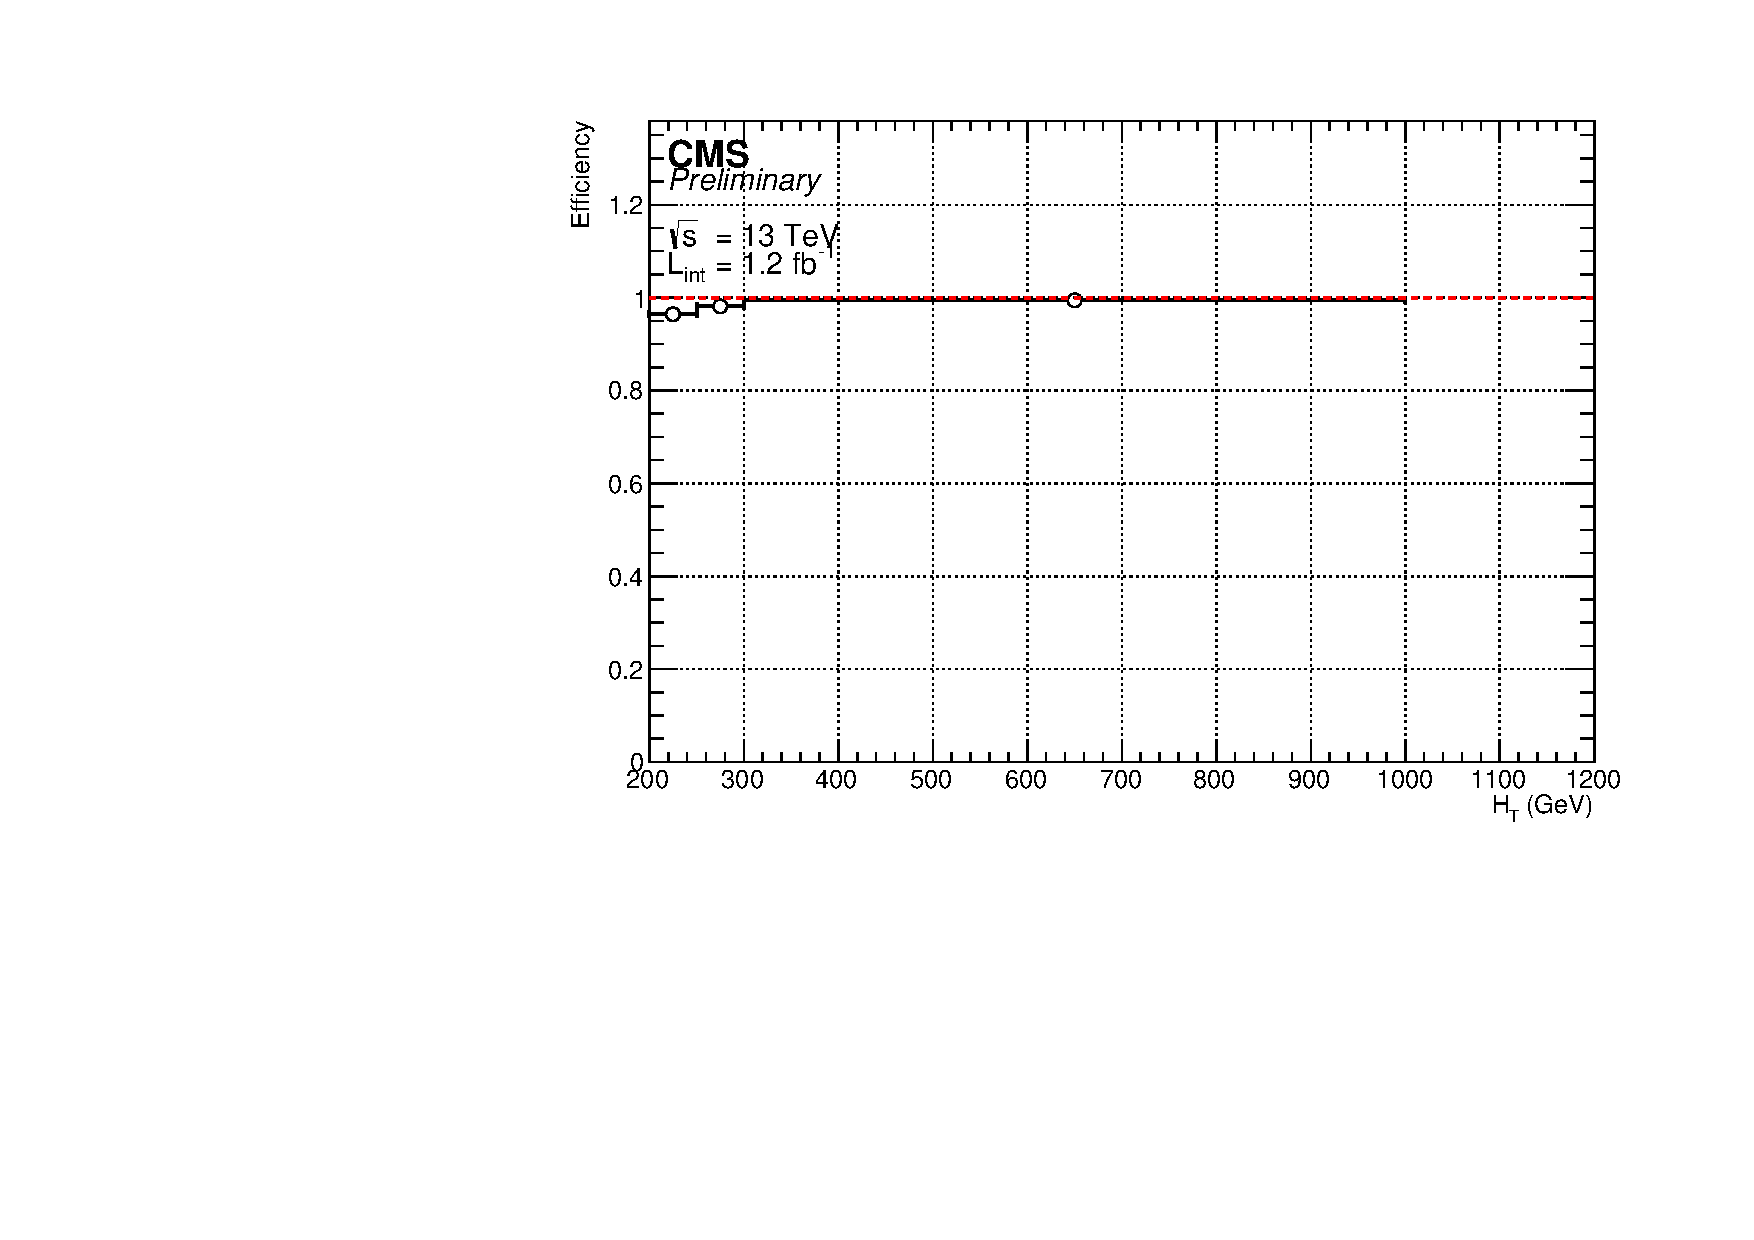
\includegraphics[width=0.5\textwidth]{figures/Trigger/HLT_IsoMu20/HLT_PFMETNoMu90_JetIdCleaned_PFMHTNoMu90_IDTight_MoM_Mono_MHT0_ht.pdf}} ~~     
%    \subfigure[Electron sample]{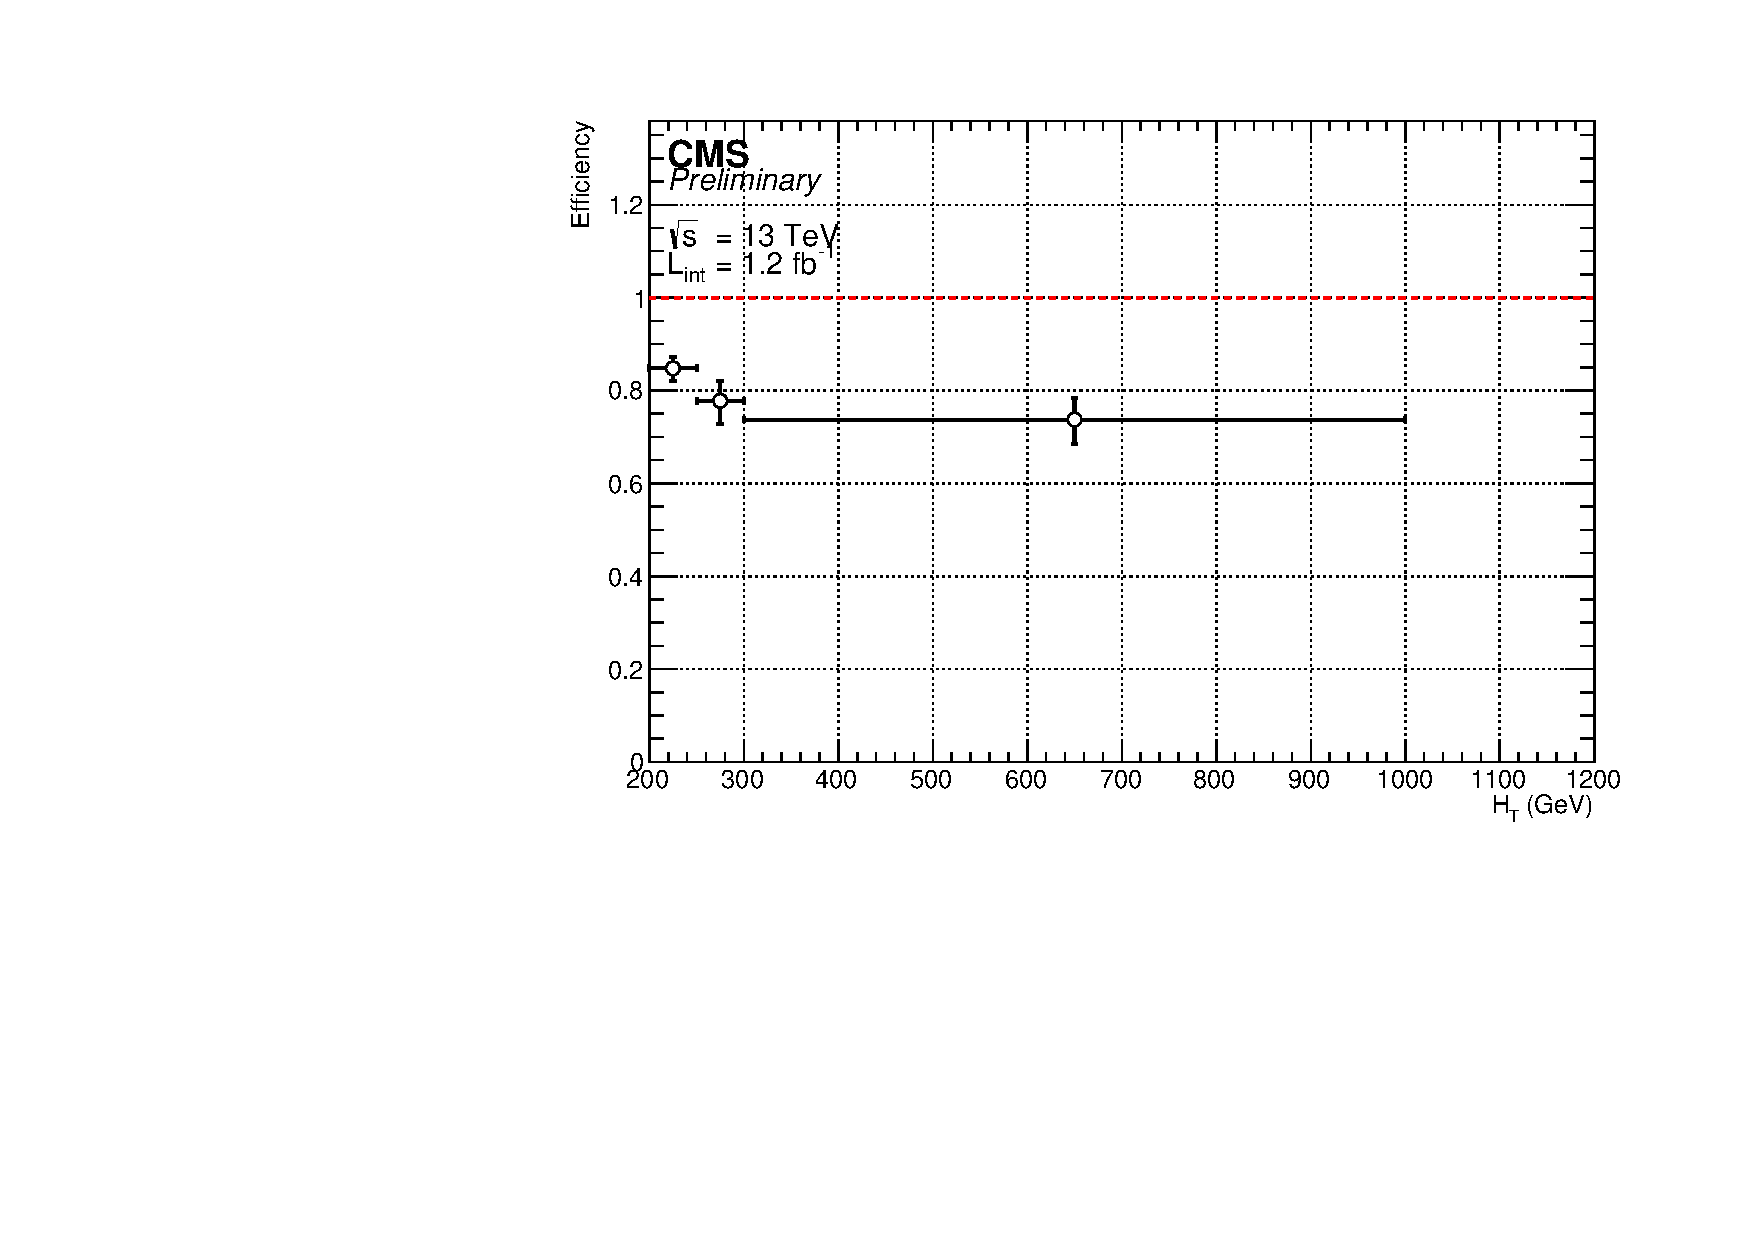
\includegraphics[width=0.5\textwidth]{figures/Trigger/HLT_Ele23_eta2p1_WPLoose_Gsf/HLT_PFMETNoMu90_JetIdCleaned_PFMHTNoMu90_IDTight_MoM_Mono_MHT0_ht.pdf}} \\
%    \caption{Trigger efficiency of the monojet trigger measured in muon and electron samples.
%          }
%    \label{fig:monojet_turnons}
%  \end{center} 
%\end{figure}


%The multijet triggers do not have the muon cross-cleaning applied online so their efficiency measurement in data 
%is primarily performed with the use of an electron sample. To remain consistent with the 
%reconstruction of electrons in the trigger, no cross-cleaning of electrons from jets 
%are performed offline, with the electron being included in the computation of event-level jet energy sums, such as 
%\scalht, \MHT and \alt. The turn-on for the individual \scalht-\alphat triggers are shown in Appendix~\ref{app:alphaTTriggerEfficiencies}

The trigger efficiency of the multijet triggers as a function of \mht after a full signal selection 
is shown in Figs.~\ref{fig:alphat_turnons_sym},\ref{fig:alphat_turnons_asym},\ref{fig:alphat_turnons_mono}, and is shown to be close to or at the plateau when taking 
the disjunction of triggers. These efficiencies are measured in bins of \scalht and \mht
per jet topology (monojet, symmetric and asymmetric). The measured
efficiencies and their uncertainties are applied as corrections to the MC
samples. The central value of the correction is taken from the efficiency
measured with the muon reference trigger. The difference in efficiencies between
those measured with the electron and muon triggers
%, together with the
%statistical uncertainty of the muon measurement, 
is propagated as a systematic
uncertainty. The efficiencies have also been checked in bins of \njet and show
no significant dependence on \njet (see Appendix~\ref{app:alphaTTriggerEfficiencies}).
%for \scalht < 800 \GeV. The efficiency without a proper cross-cleaning
%is predicted to be exceed that measured with electron bias. A full efficiency is therefore assumed for 
%these triggers with a systematic to this estimate assigned equal to the
%inefficiency estimated by the respective reference trigger. 
%For \scalht $> 800$ \GeV, where the bias of electrons is a smaller effect, the trigger 
%efficiency is measured for the disjunction of the \scalht-\alphat and \verb!HLT_HT800! triggers, inclusively on jet multiplicity, and a correction applied which is shown in Fig.~\ref{fig:ht800_turnons}. 

The turn-ons for the individual \scalht-\alphat triggers are shown in
Appendix~\ref{app:alphaTTriggerEfficiencies}.

\begin{figure}[h!]
  \begin{center}
    \subfigure[$200 < \scalht < 250$]{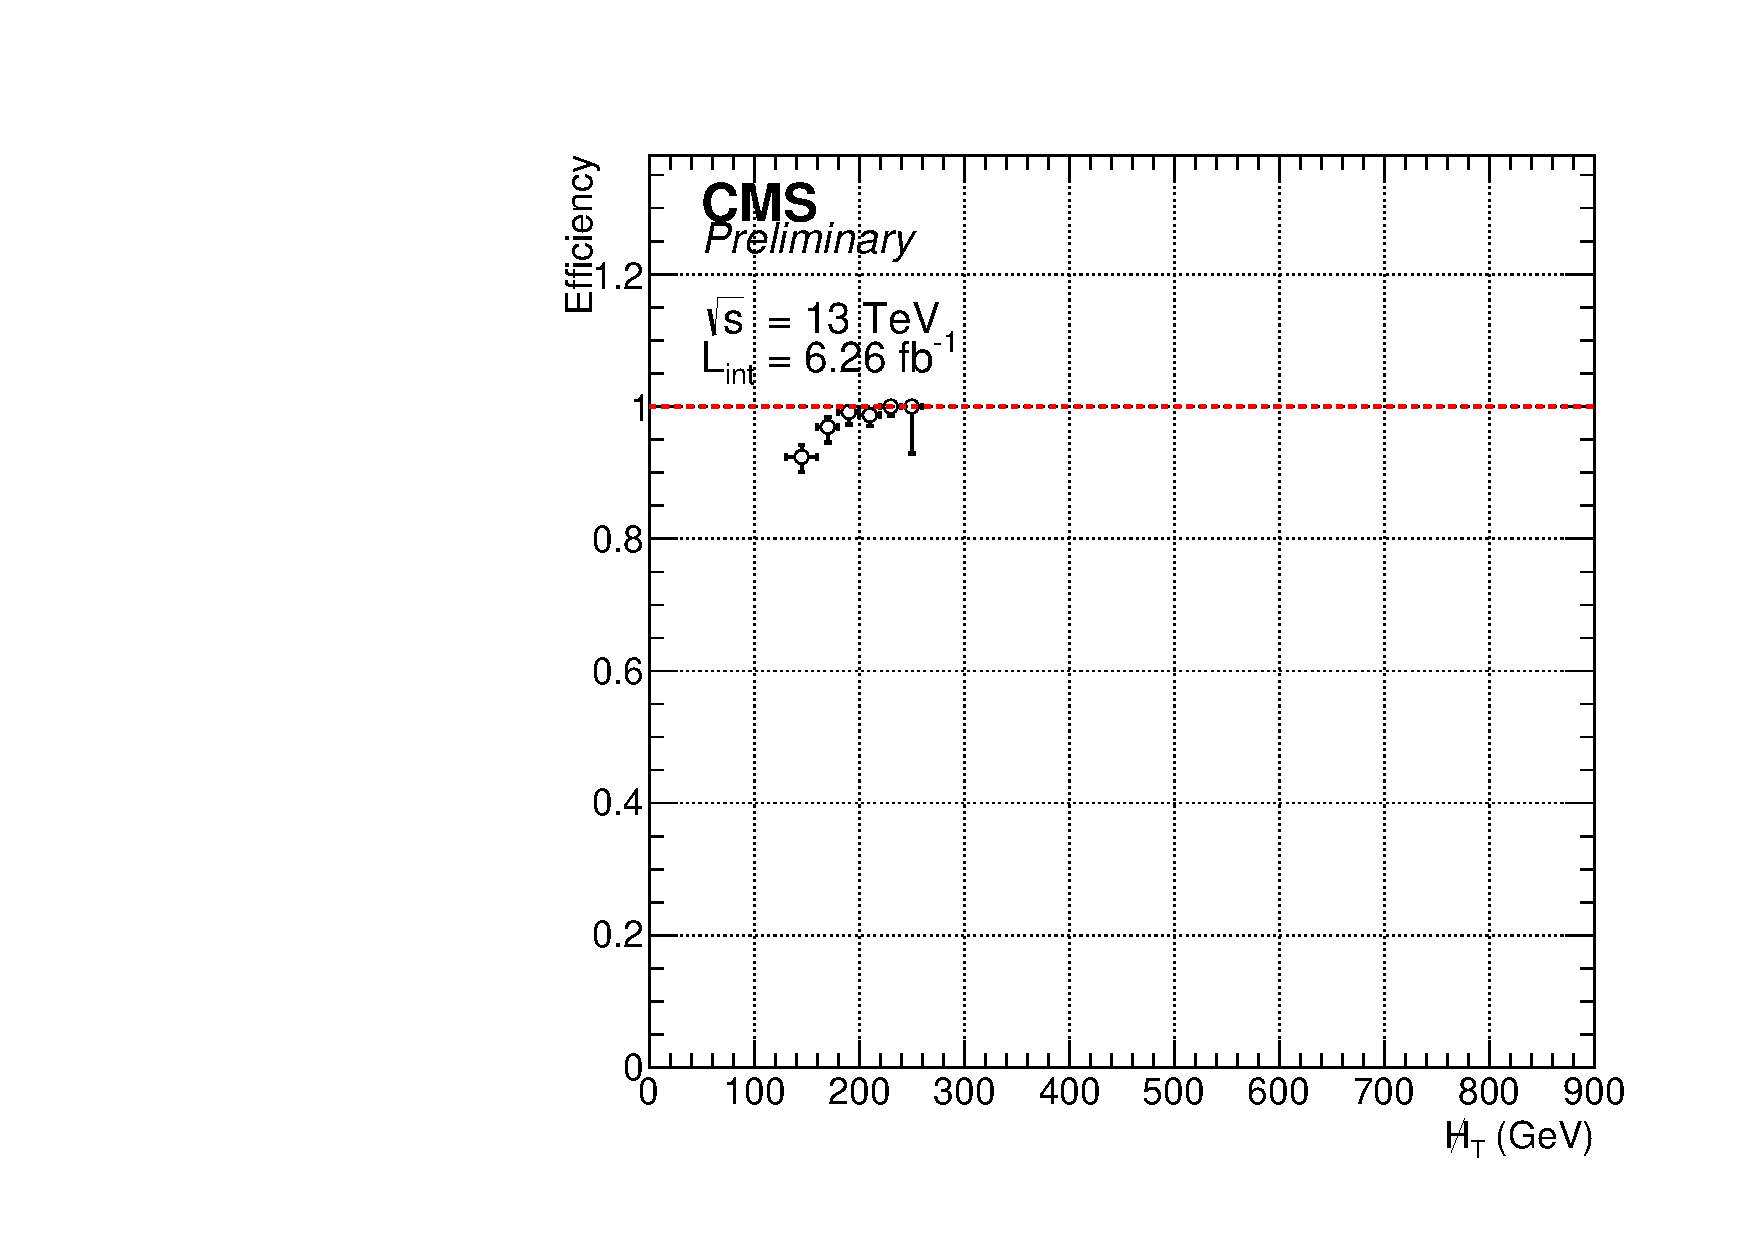
\includegraphics[width=0.4\textwidth]{figures/Trigger/HLT_IsoMu22/HLT_AlphaTMonoAll_MoM_200to250_mht}} ~~\
    \subfigure[$300 < \scalht < 350$]{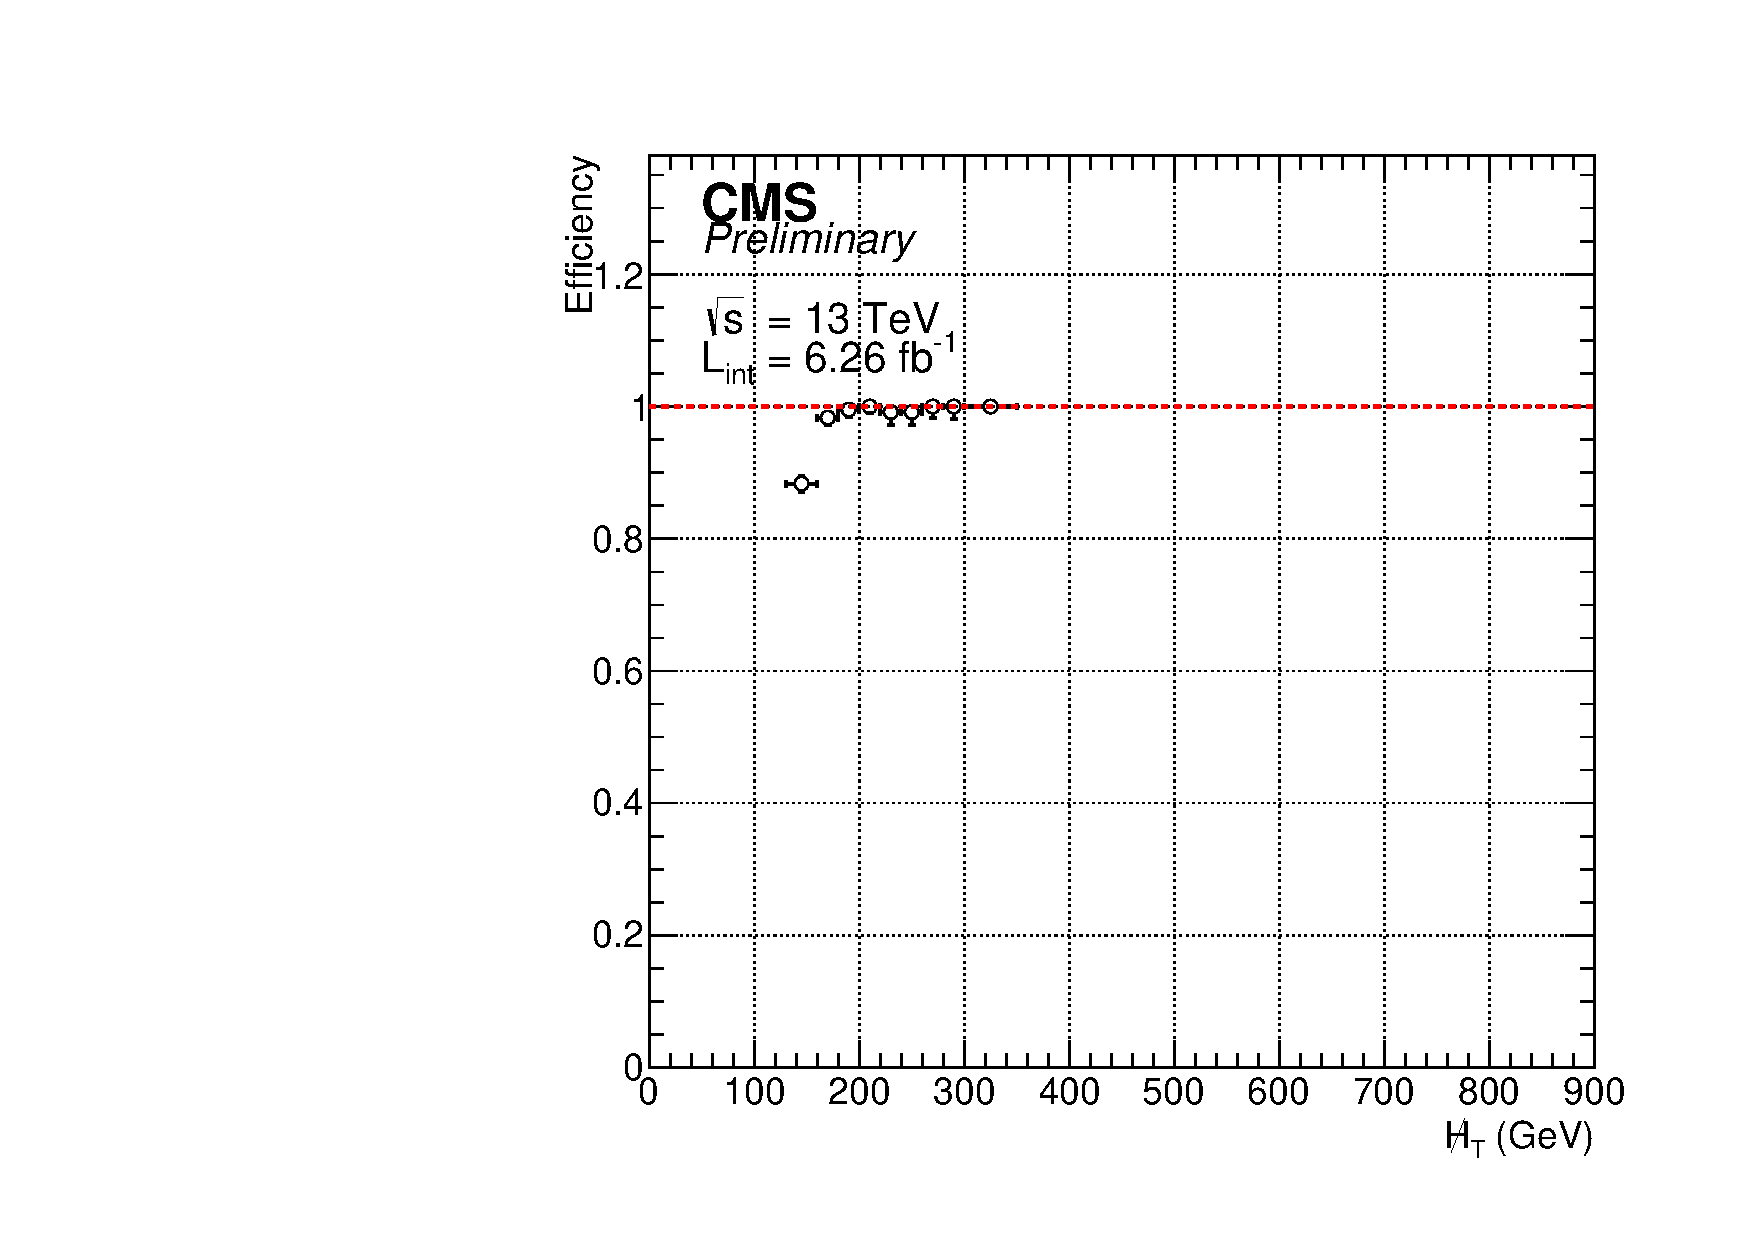
\includegraphics[width=0.4\textwidth]{figures/Trigger/HLT_IsoMu22/HLT_AlphaTMonoAll_MoM_300to350_mht}} \\
    \subfigure[$400 < \scalht < 600$]{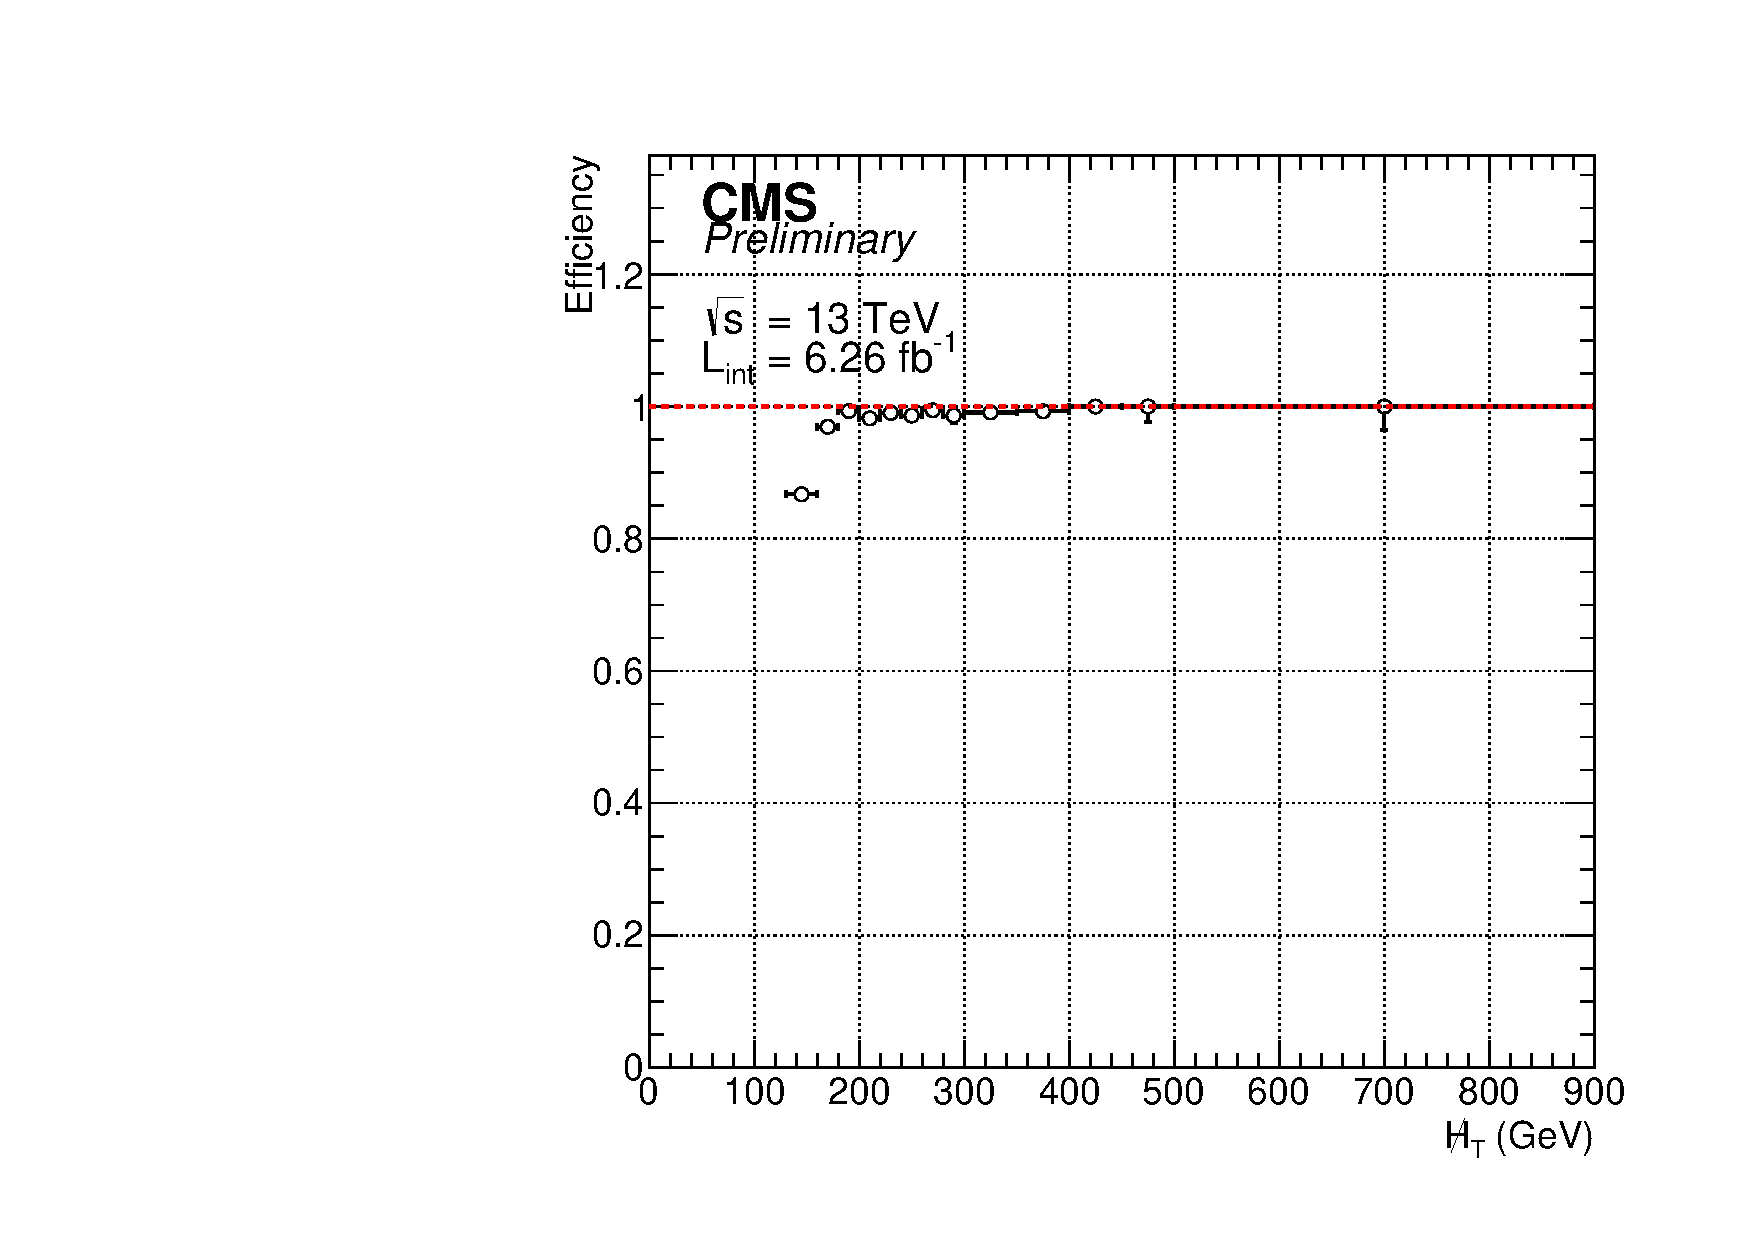
\includegraphics[width=0.4\textwidth]{figures/Trigger/HLT_IsoMu22/HLT_AlphaTMonoAll_MoM_400to600_mht}} ~~\
    \subfigure[$600 < \scalht < 800$]{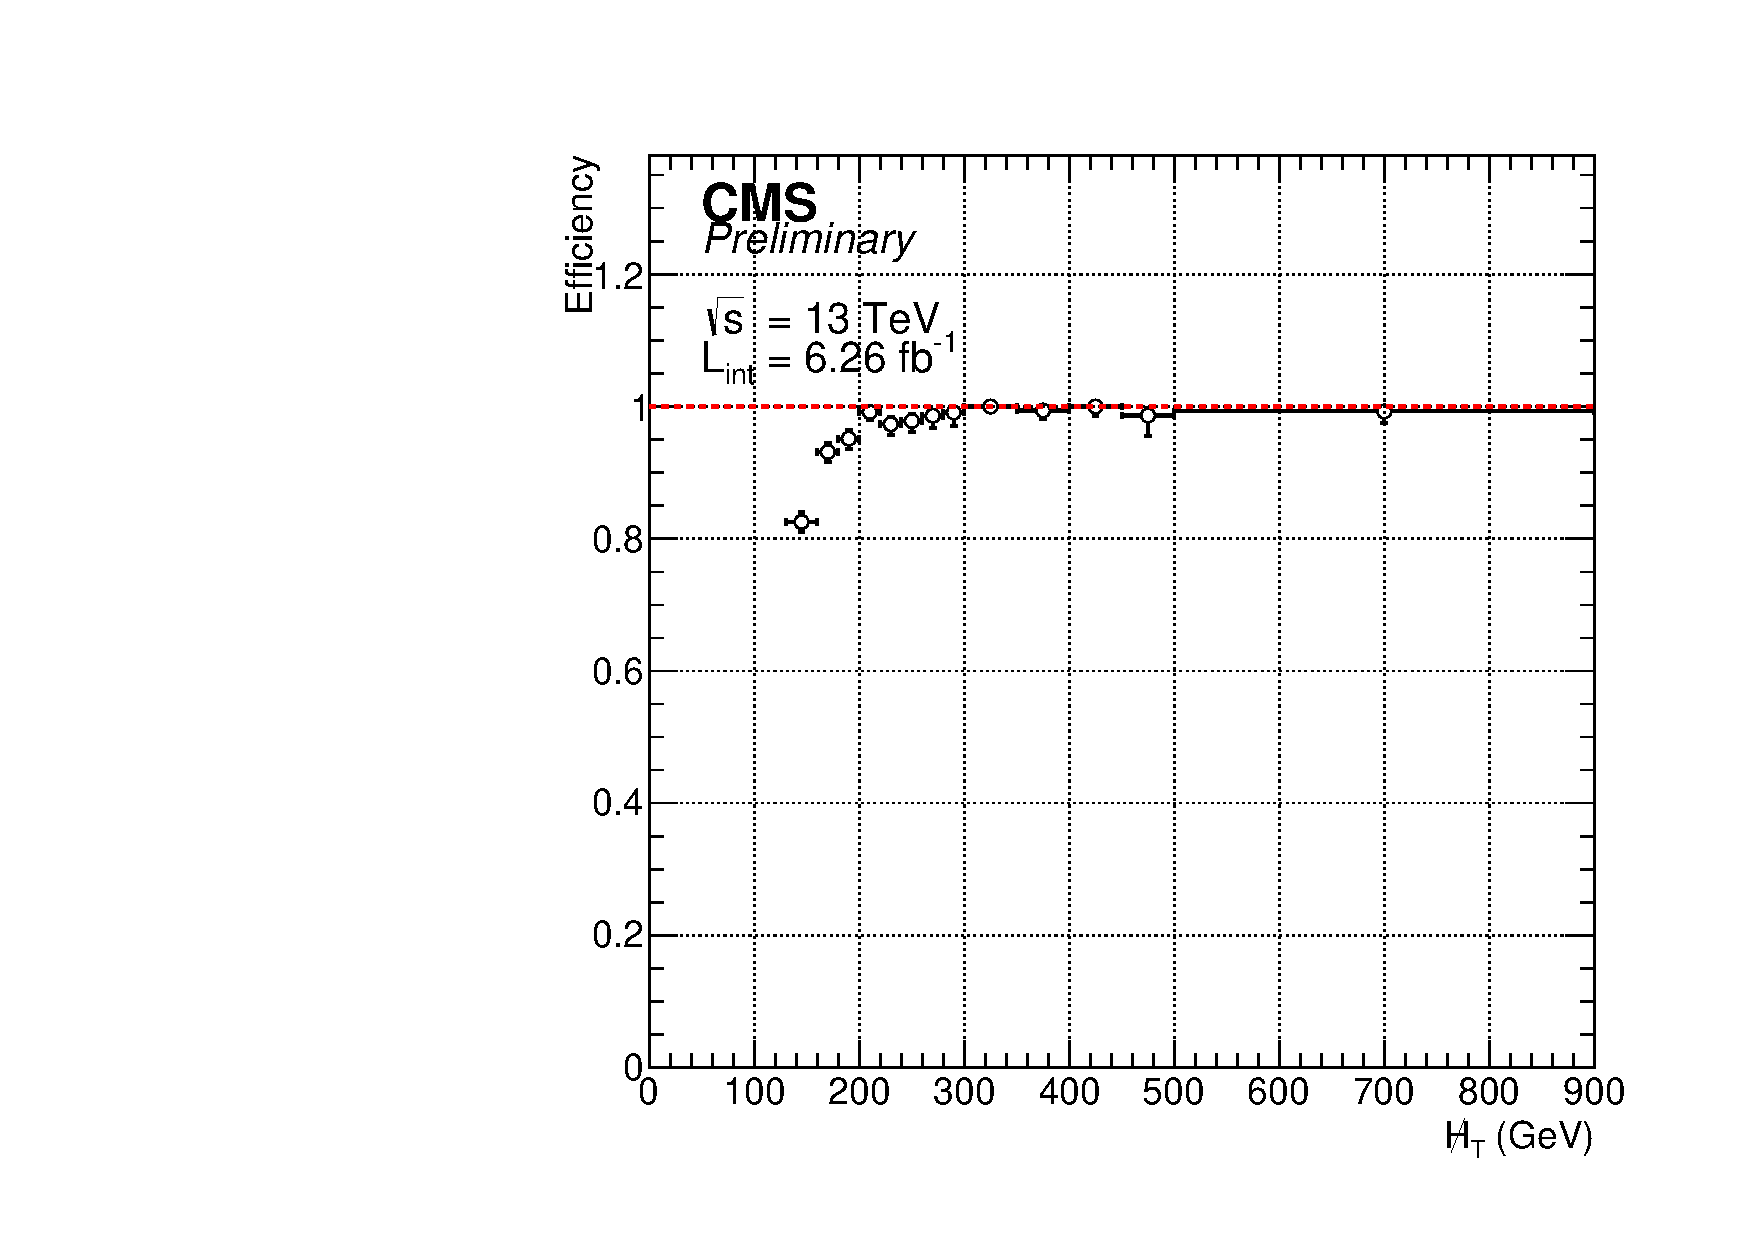
\includegraphics[width=0.4\textwidth]{figures/Trigger/HLT_IsoMu22/HLT_AlphaTMonoAll_MoM_600to800_mht}} \\
    \subfigure[$\scalht > 800$]{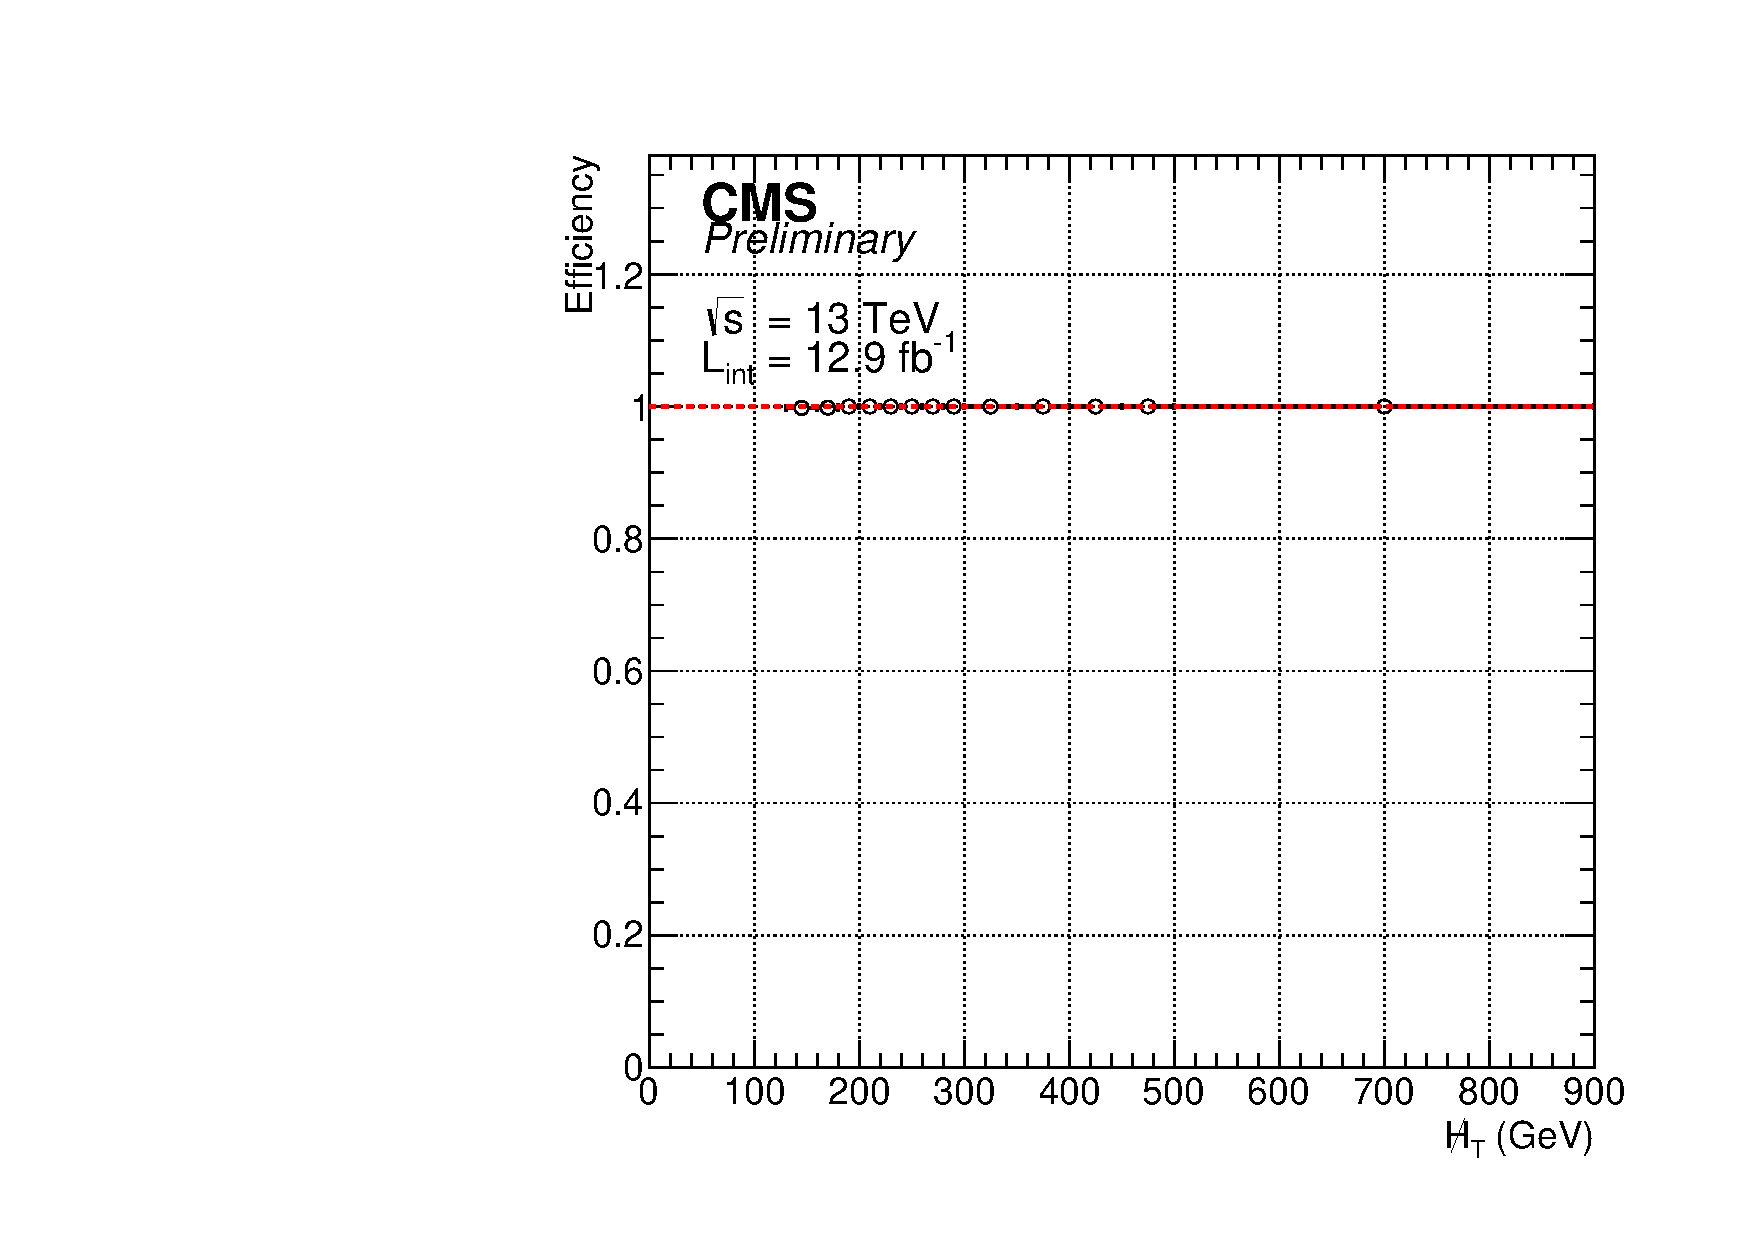
\includegraphics[width=0.4\textwidth]{figures/Trigger/HLT_IsoMu22/HLT_AlphaTHT800MonoAll_MoM_800to999999_mht}} \\ ~~\
    \caption{Signal trigger efficiency in the \mht dimension measured with a muon sample, for symmetric categories.}
    \label{fig:alphat_turnons_sym}
  \end{center}
\end{figure}

\begin{figure}[h!]
  \begin{center}
    \subfigure[$200 < \scalht < 250$]{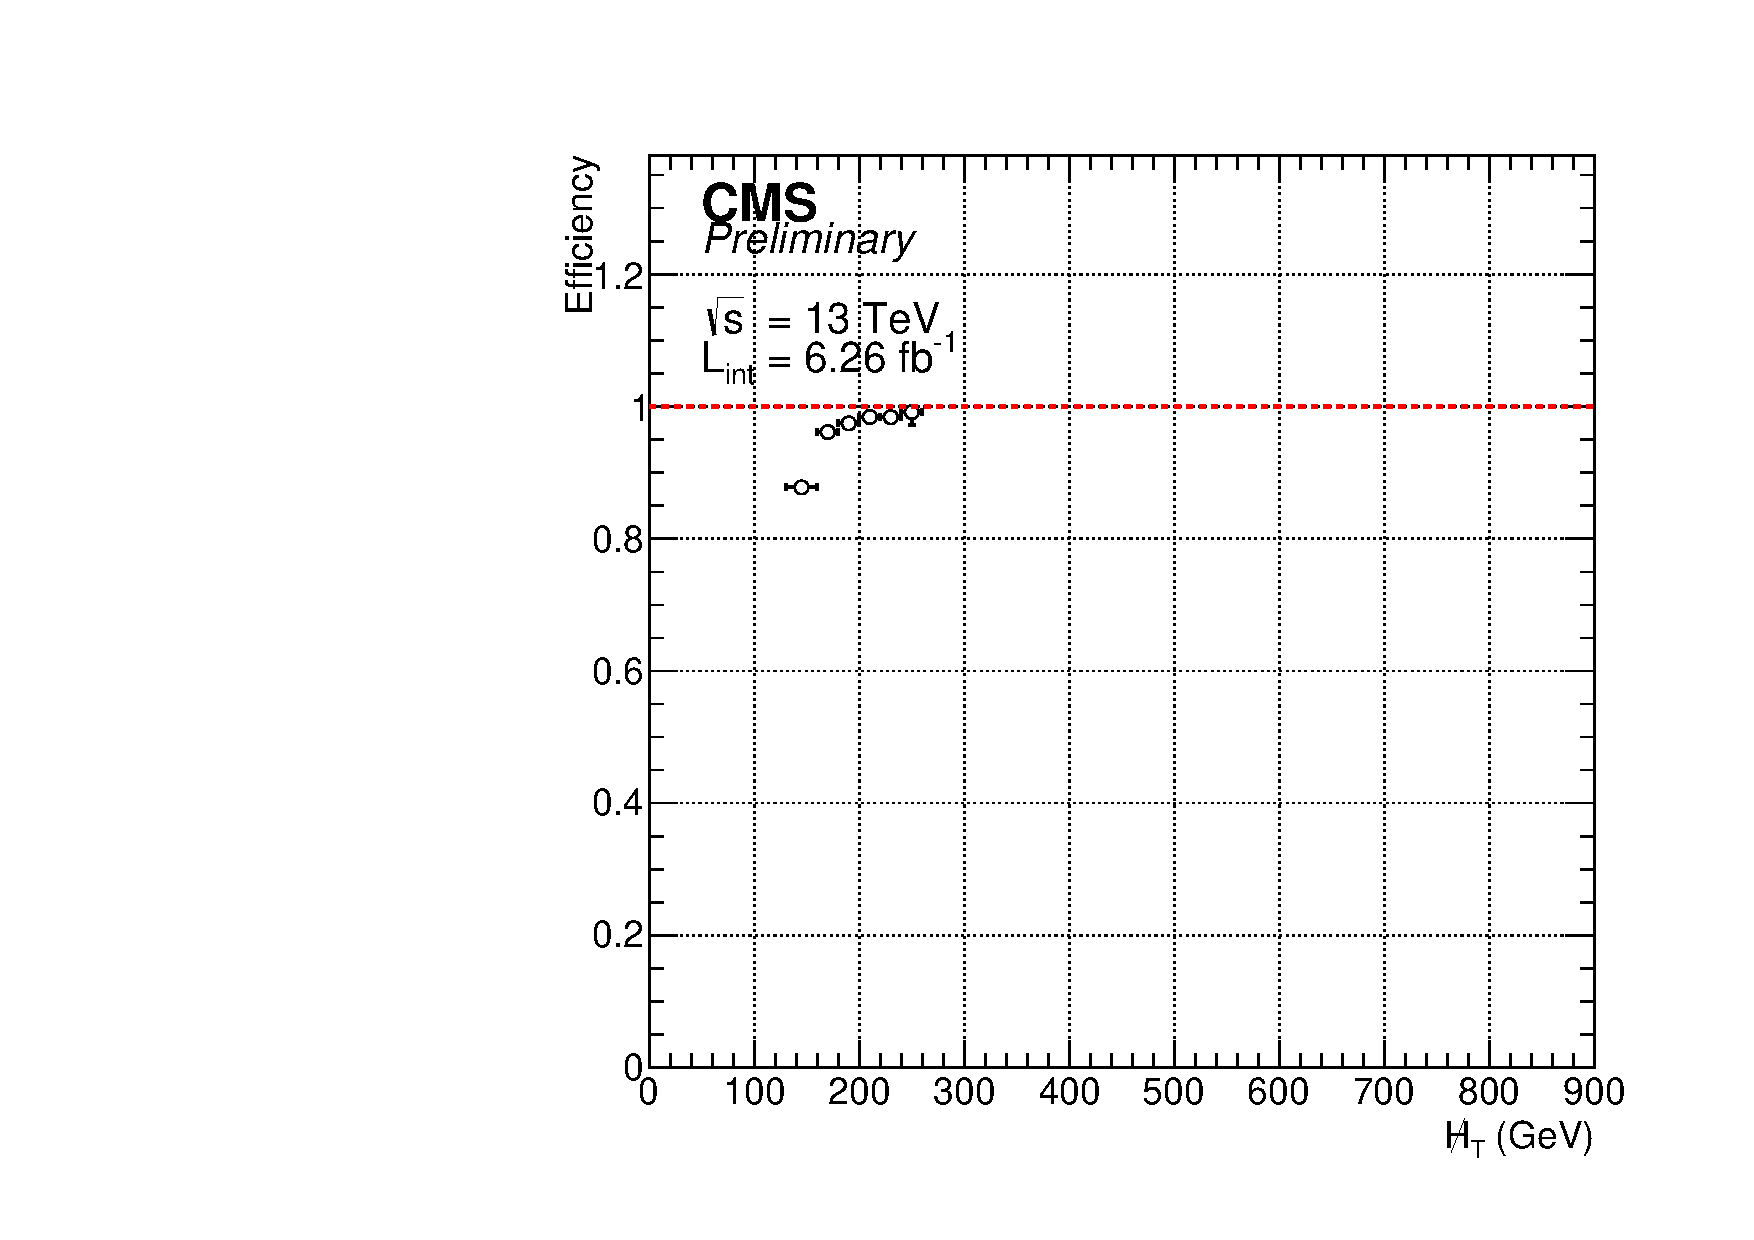
\includegraphics[width=0.4\textwidth]{figures/Trigger/HLT_IsoMu22/HLT_AlphaTMonoAll_MoM_Asym_200to250_mht}} ~~\
    \subfigure[$300 < \scalht < 350$]{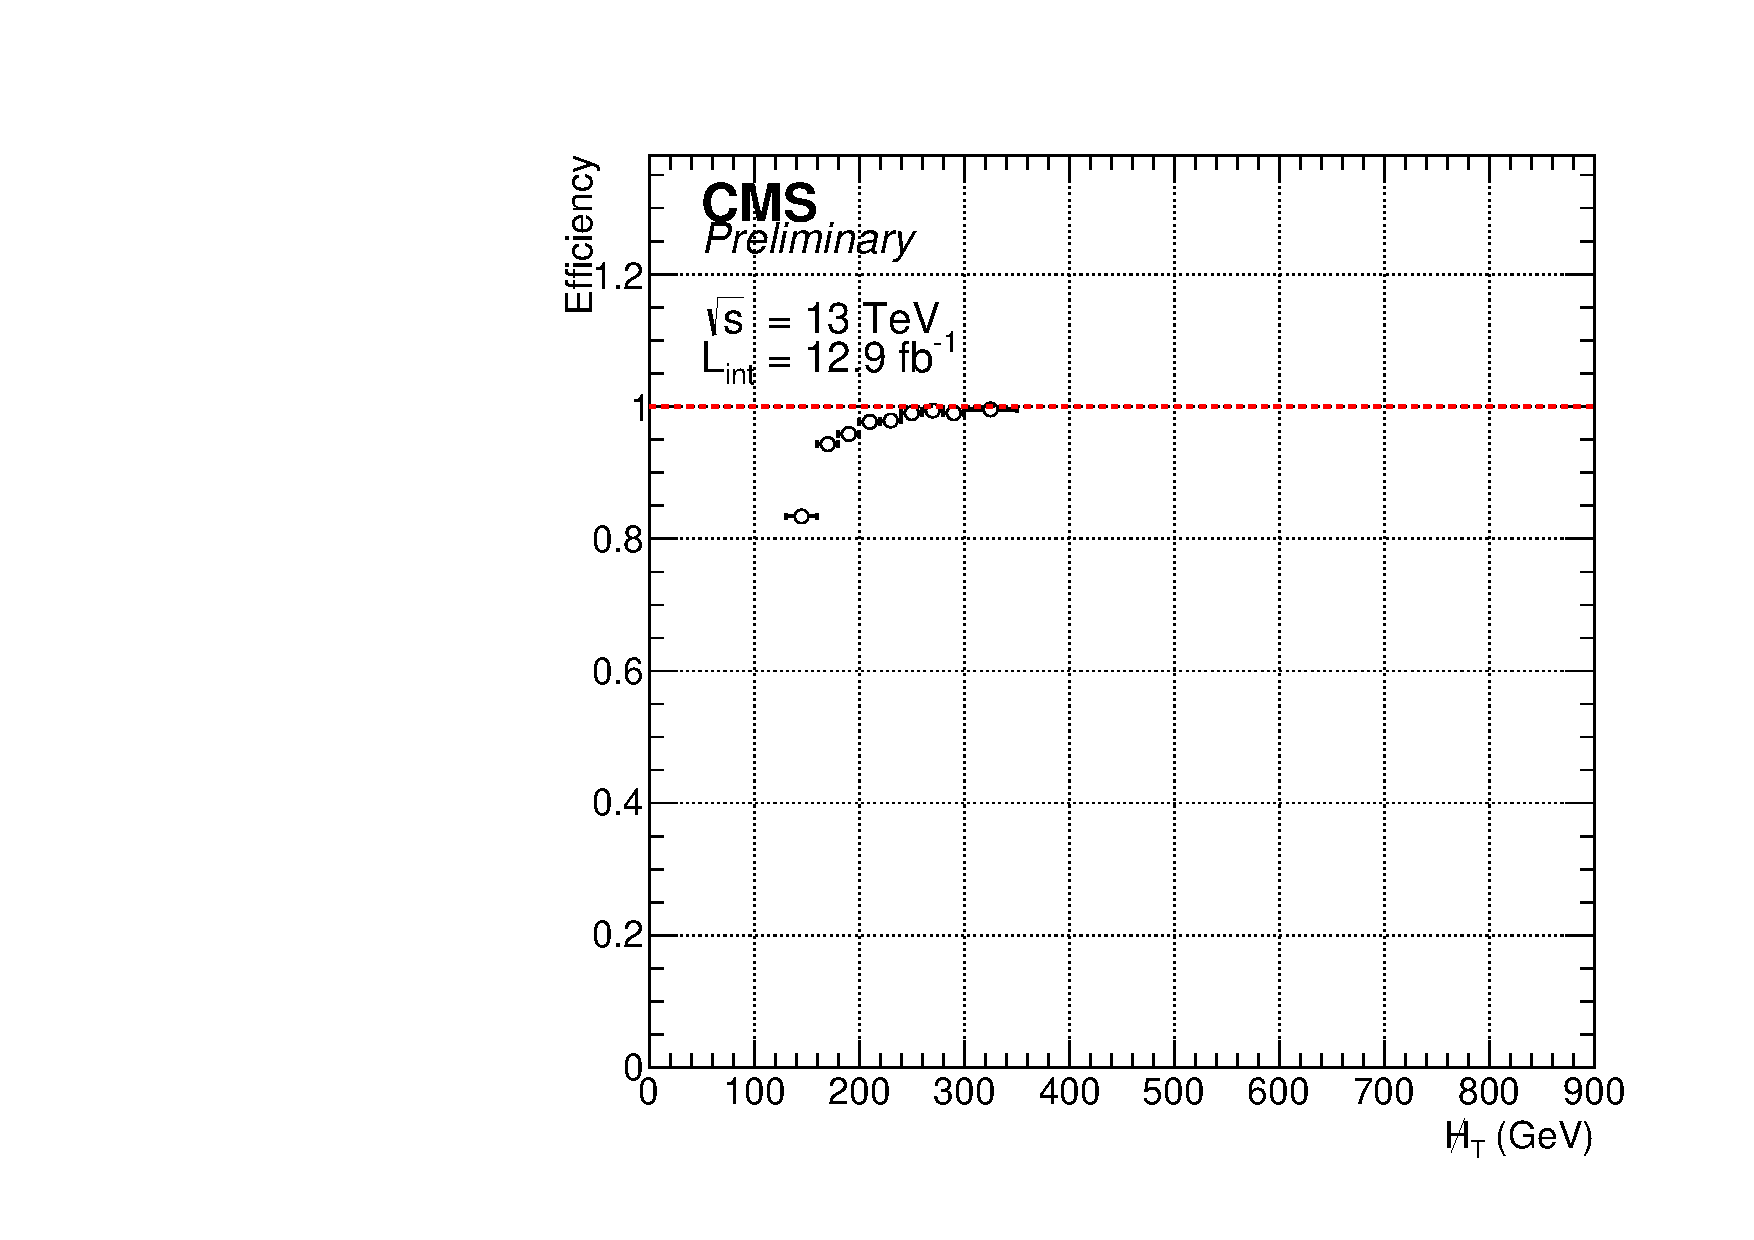
\includegraphics[width=0.4\textwidth]{figures/Trigger/HLT_IsoMu22/HLT_AlphaTMonoAll_MoM_Asym_300to350_mht}} \\
    \subfigure[$400 < \scalht < 600$]{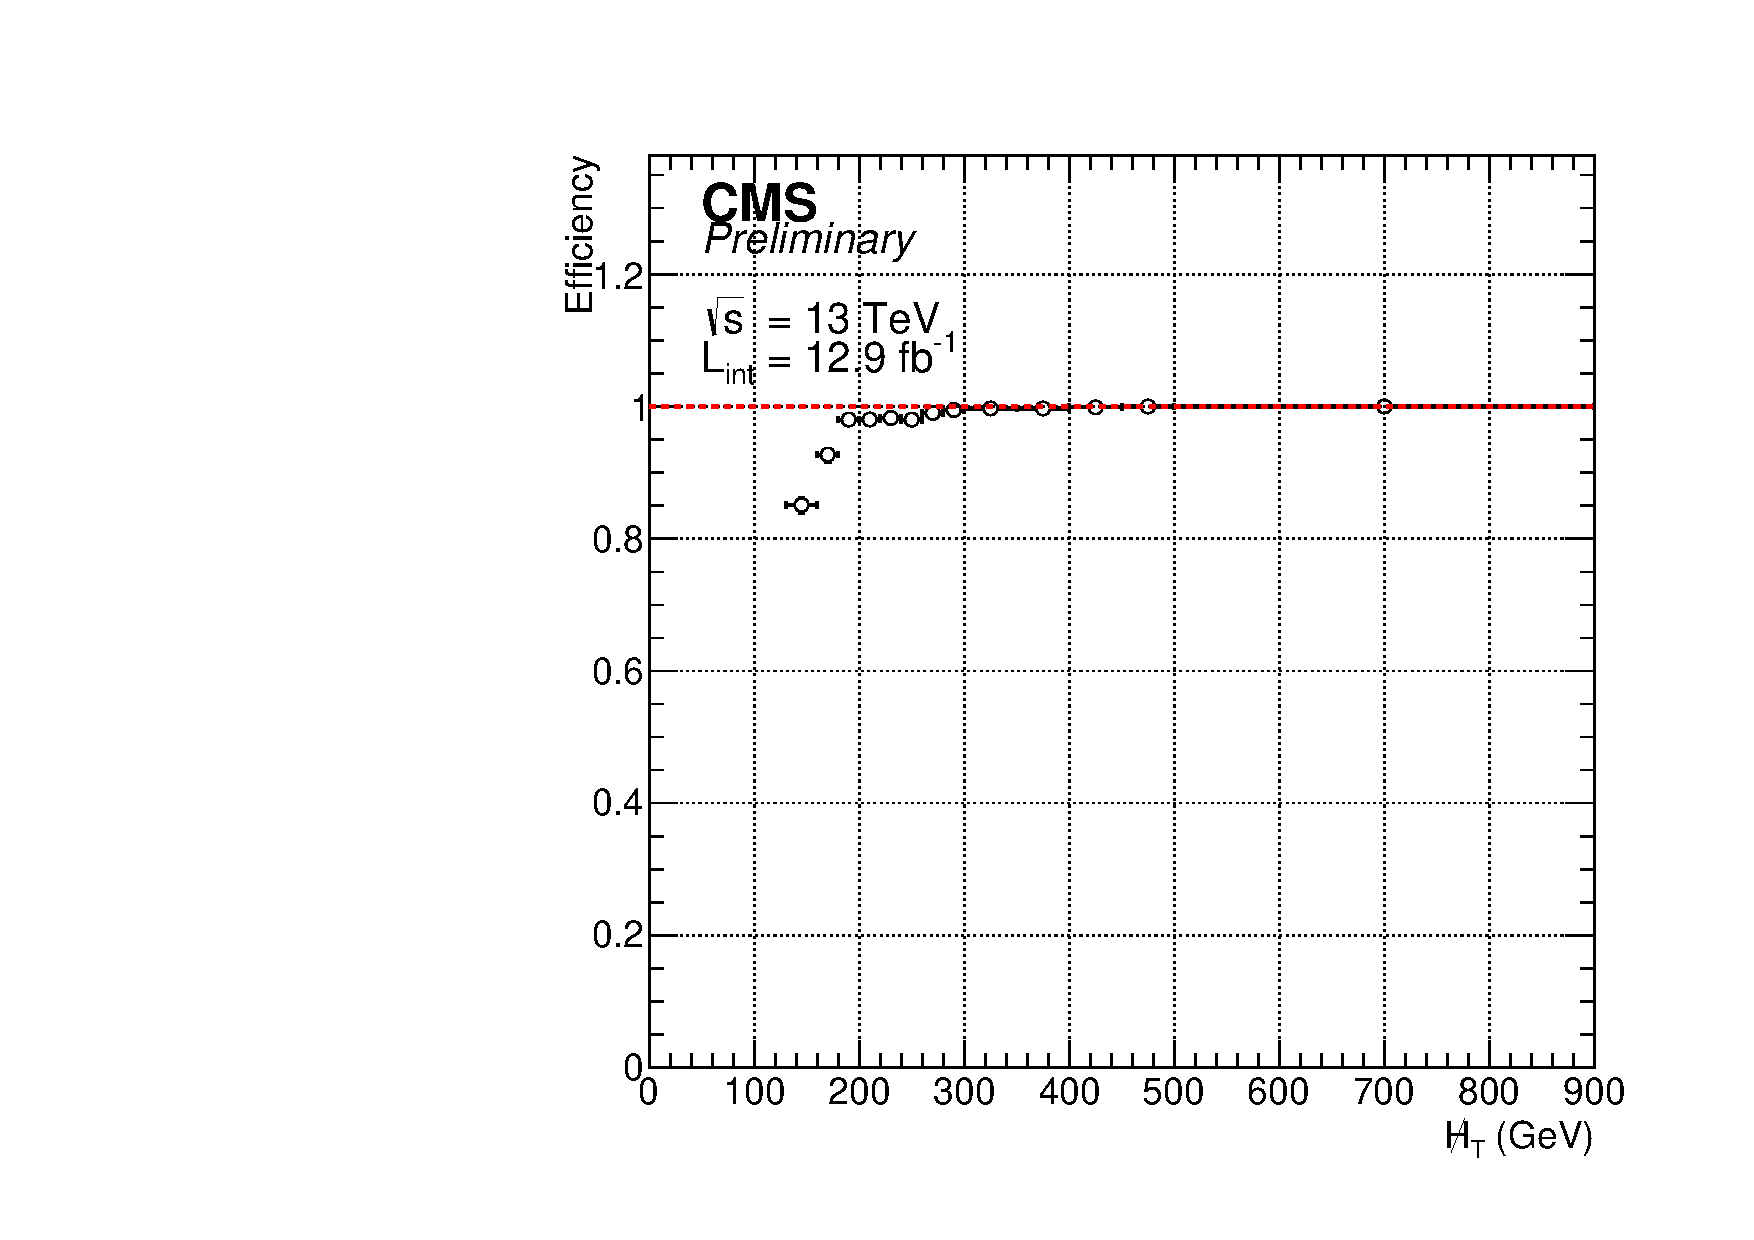
\includegraphics[width=0.4\textwidth]{figures/Trigger/HLT_IsoMu22/HLT_AlphaTMonoAll_MoM_Asym_400to600_mht}} ~~\
    \subfigure[$\scalht > 600$]{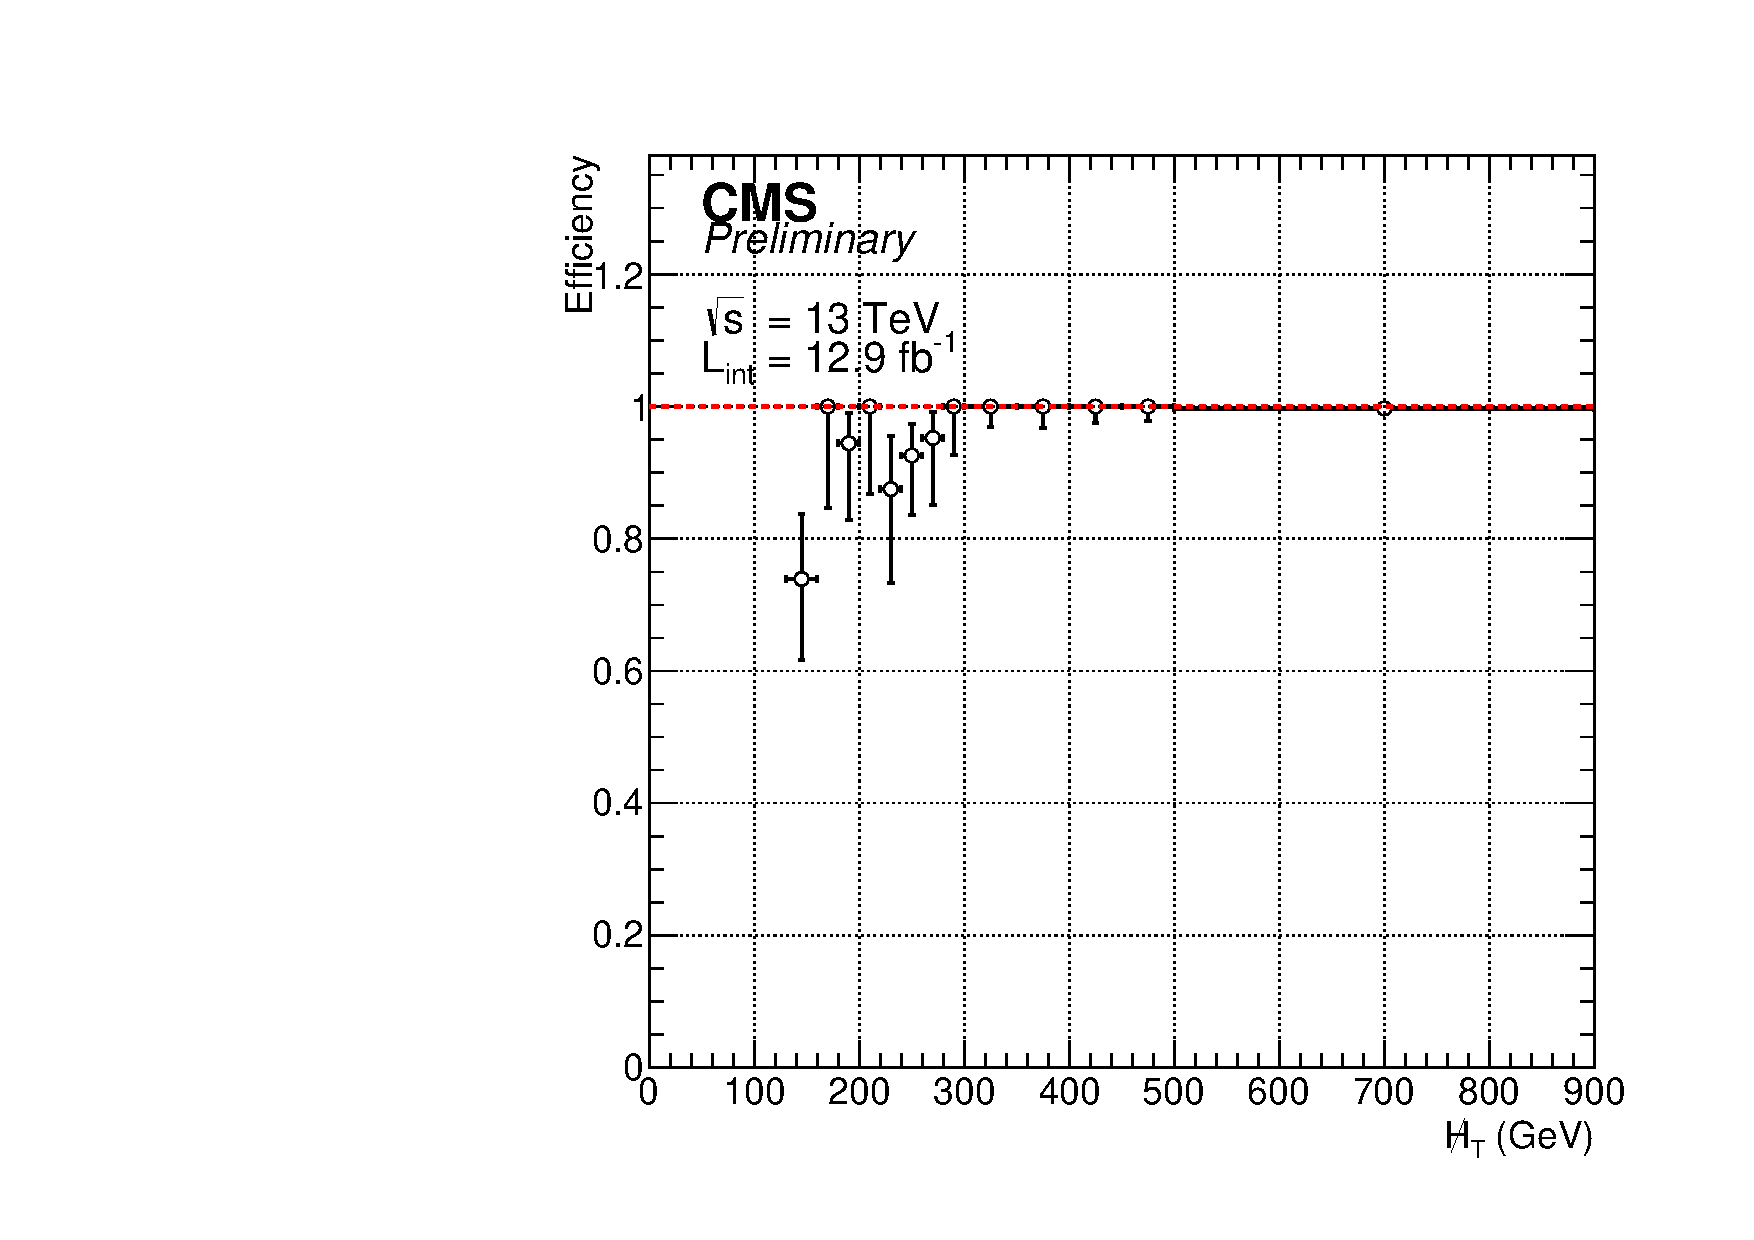
\includegraphics[width=0.4\textwidth]{figures/Trigger/HLT_IsoMu22/HLT_AlphaTMonoAll_MoM_Asym_600to999999_mht}} \\
    \caption{Signal trigger efficiency in the \mht dimension measured with a muon sample, for asymmetric categories.}
    \label{fig:alphat_turnons_asym}
  \end{center}
\end{figure}

\begin{figure}[h!]
  \begin{center}
    \subfigure{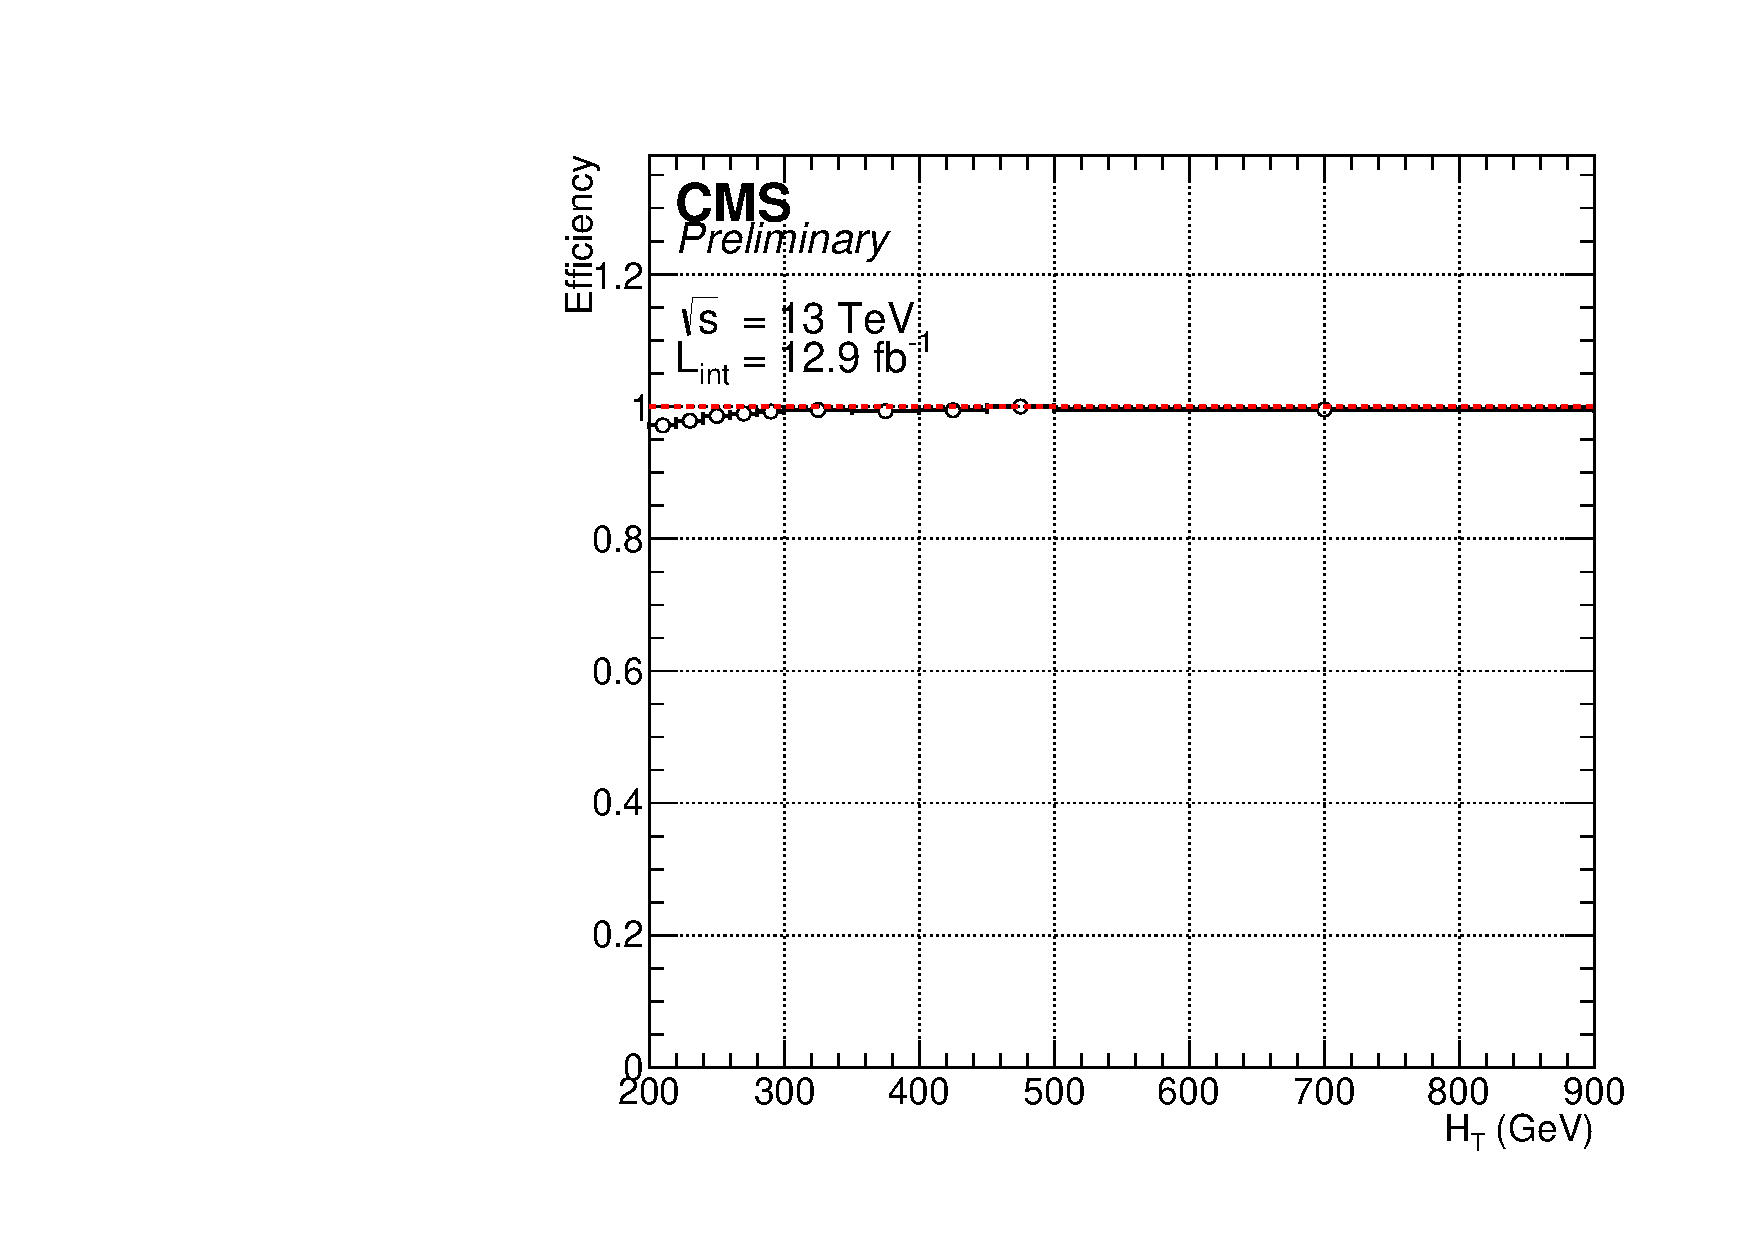
\includegraphics[width=0.4\textwidth]{figures/Trigger/HLT_IsoMu22/HLT_MonoAll_MoM_Mono_MHT0_ht}} \\
    \caption{Signal trigger efficiency in the \mht$=$\scalht dimension measured with a muon sample, for monojet categories.}
    \label{fig:alphat_turnons_mono}
  \end{center}
\end{figure}



%\newpage

% Control region triggers
\subsection{Control regions\label{sec:control_samples}}
%Prescaled $\scalht$ triggers, \verb!HLT_PFHTXXX!, and a prescaled 
%$\scalht$-$\alphat$ cross-trigger, are utilised in the 
%selection of events for the hadronic control region. Shown 
%in Table~\ref{tab:2015_Hadronic_Control_Triggers} these triggers share the same Level-1 
%seeds and $\scalht$ threshold of the signal cross-triggers and are similarly each mapped 
%to a unique offline bin. The efficiency of these triggers are similarly measured from an electron 
%reference trigger in addition to an independent measurement with the \verb!HLT_Physics! 
%minimum bias trigger.


% TABLE: Hadronic control region
%\begin{table}[h!]
%\topcaption{Hadronic control triggers. }
%\footnotesize
%\centering
%\begin{tabular}{c|cc} 
%\hline
%\hline
%HLT path & \multicolumn{1}{c}{Prescale} \\
%\hline
%\texttt{HLT\_PFHT200} & 3060 \\
%\texttt{HLT\_PFHT250} & 2040 \\
%\texttt{HLT\_PFHT300} & 1020 \\
%\texttt{HLT\_PFHT350} & 180  \\
%\texttt{HLT\_PFHT400} & 120  \\
%\texttt{HLT\_PFHT200\_PFAlphaT0p51} & 175 \\
%\hline
%\hline
%\end{tabular}
%\label{tab:2015_Hadronic_Control_Triggers}
%\end{table}


The non-hadronic control regions are seeded by the lowest-threshold unprescaled 
triggers available in the given run scenario. The 
\mj and \mmj control samples are selected with the logical OR of the \verb!HLT_IsoMu22!
and \verb!HLT_IsoTkMu22! triggers.
The efficiency is measured in data by the muon POG using the tag and probe method,
and corrections are applied to the MC samples as a function of muon \Pt and $\eta$.

The \gj control sample is selected by the OR of the \verb!HLT_Photon175! and
\verb!HLT_ECALHT800! triggers. The efficiency is measured as a function of photon
\Pt and \mht for events in the JetHT data set satisfying the \gj control region selection,
and is show in Fig.~\ref{fig:photon_turnons}. The single photon trigger exhibits a decreasing efficiency
with increasing photon \Pt, which is attributed to an H/E cut at Level 1. The inefficiency
can be partly recovered by employing the ECALHT800 trigger. In this way, a full efficiency
is recovered by a photon \Pt of 400 GeV in the $\scalht > 800$ GeV bin. These efficiencies are used
to correct the MC samples, and a systematic uncertainty with a size of the 
inefficiency is assigned.

\begin{figure}[h!]
  \begin{center}
    \subfigure{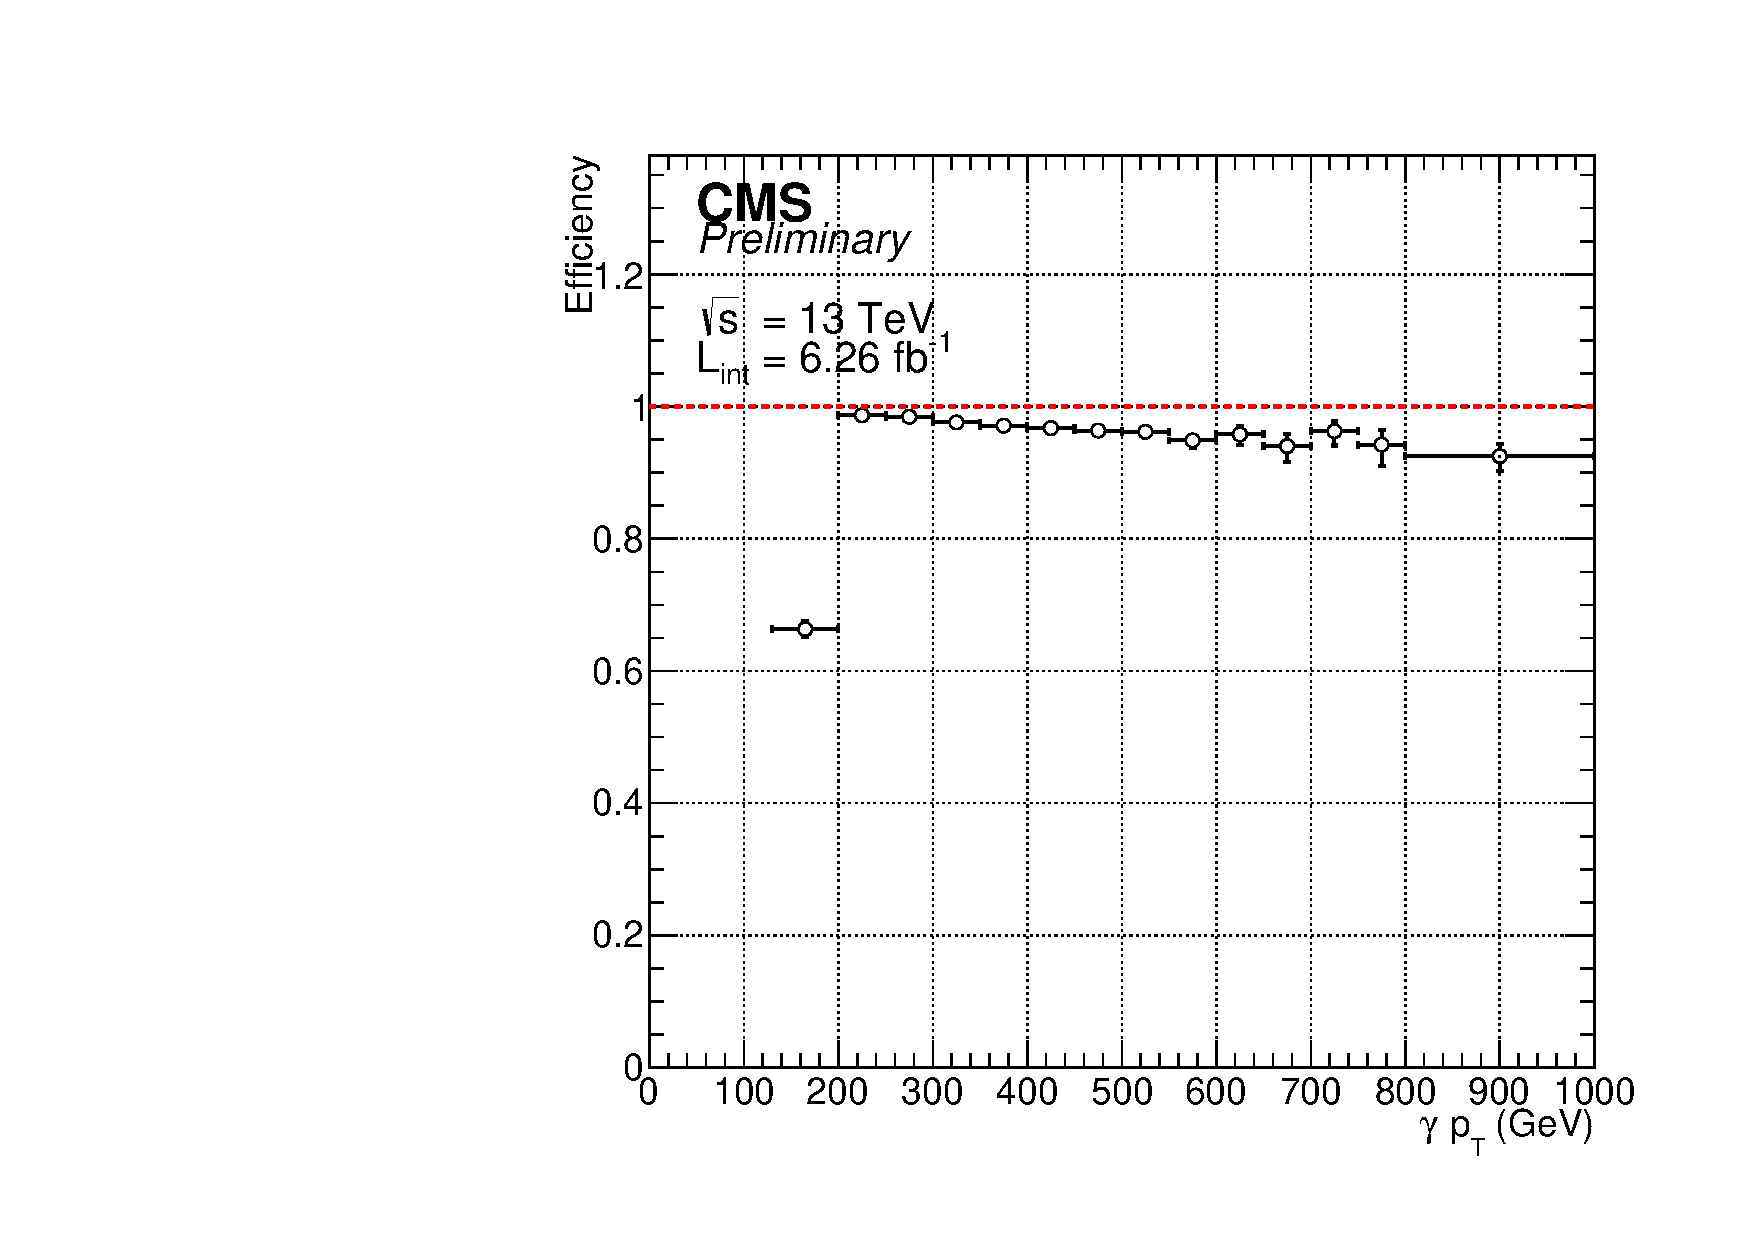
\includegraphics[width=0.4\textwidth]{figures/Trigger/Photon/HLT_Photon175_MoM_all_all_gammapt}} ~~\
    \subfigure{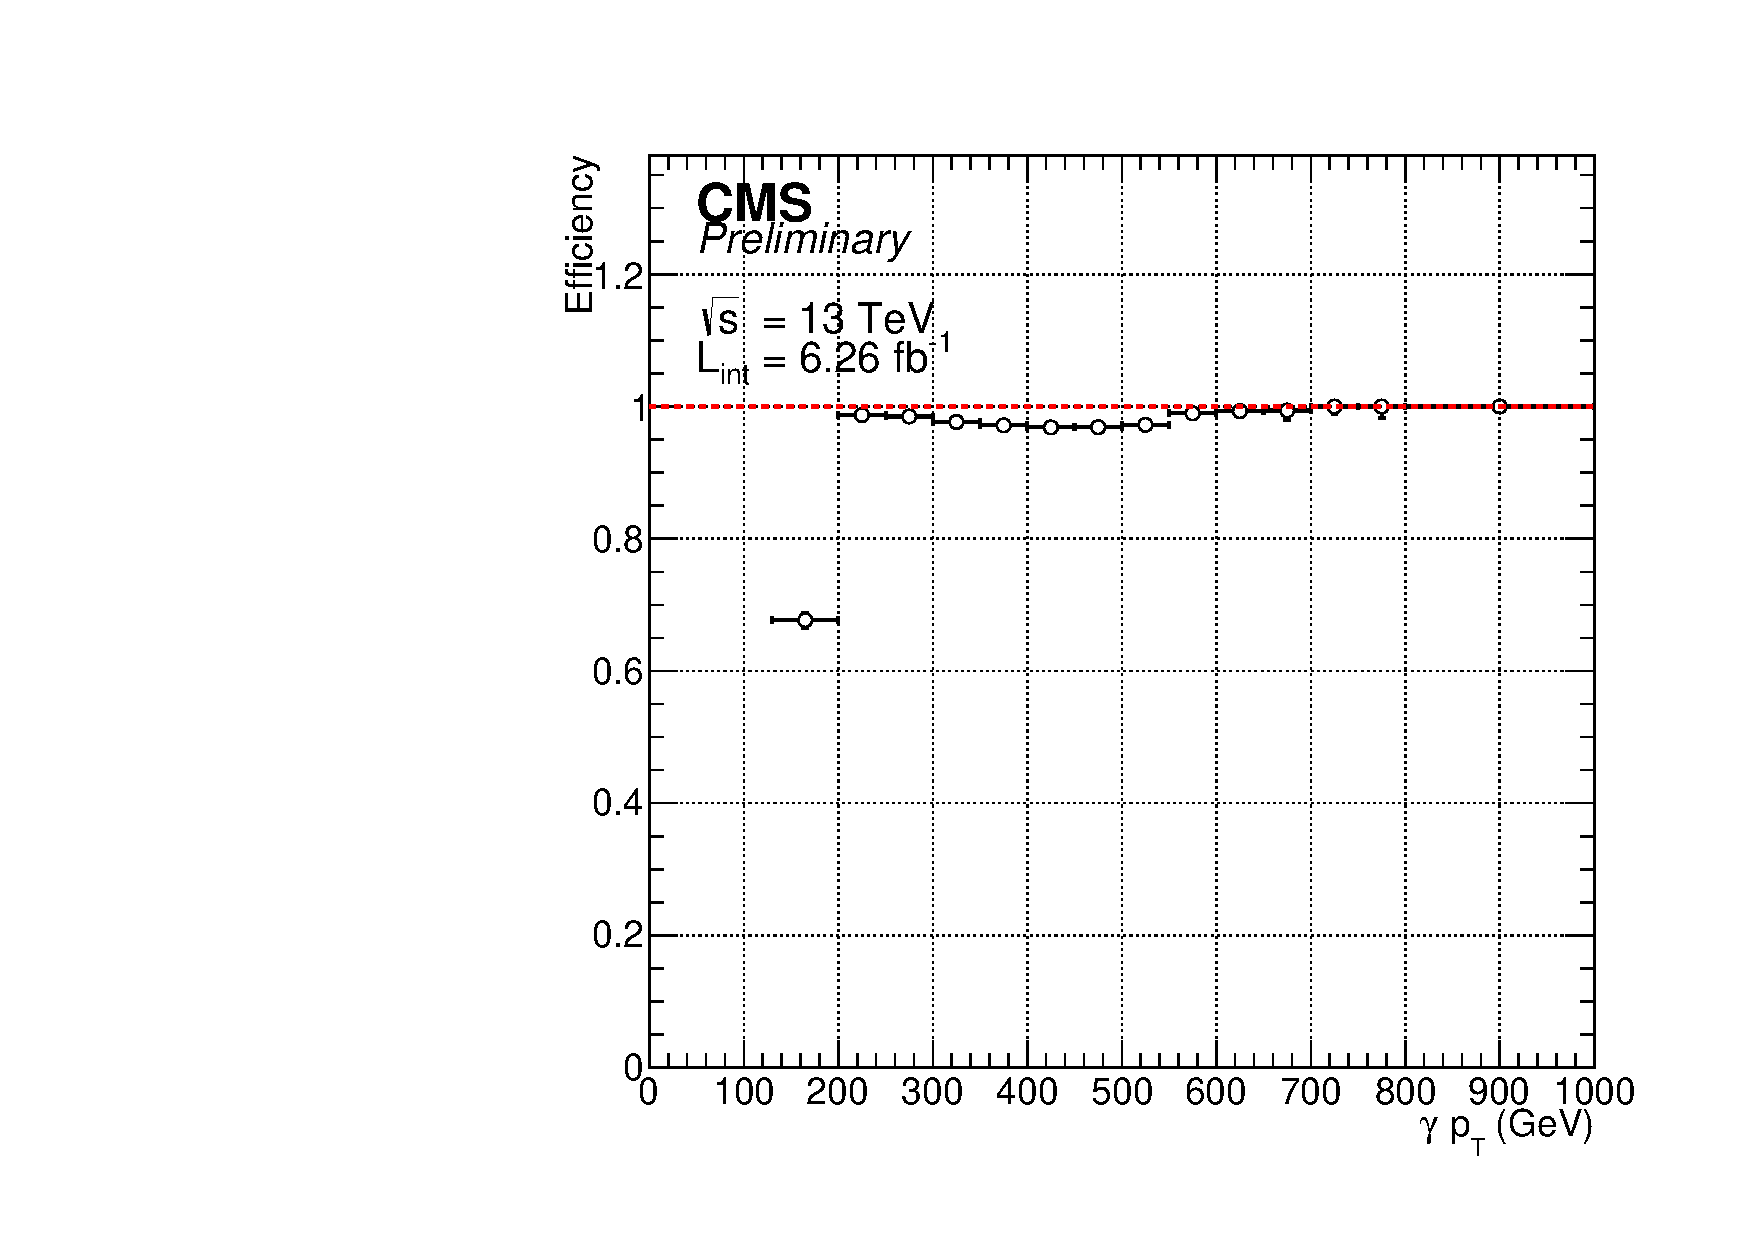
\includegraphics[width=0.4\textwidth]{figures/Trigger/Photon/HLT_PhotonECALHT800_MoM_all_all_gammapt}} \\
    \subfigure{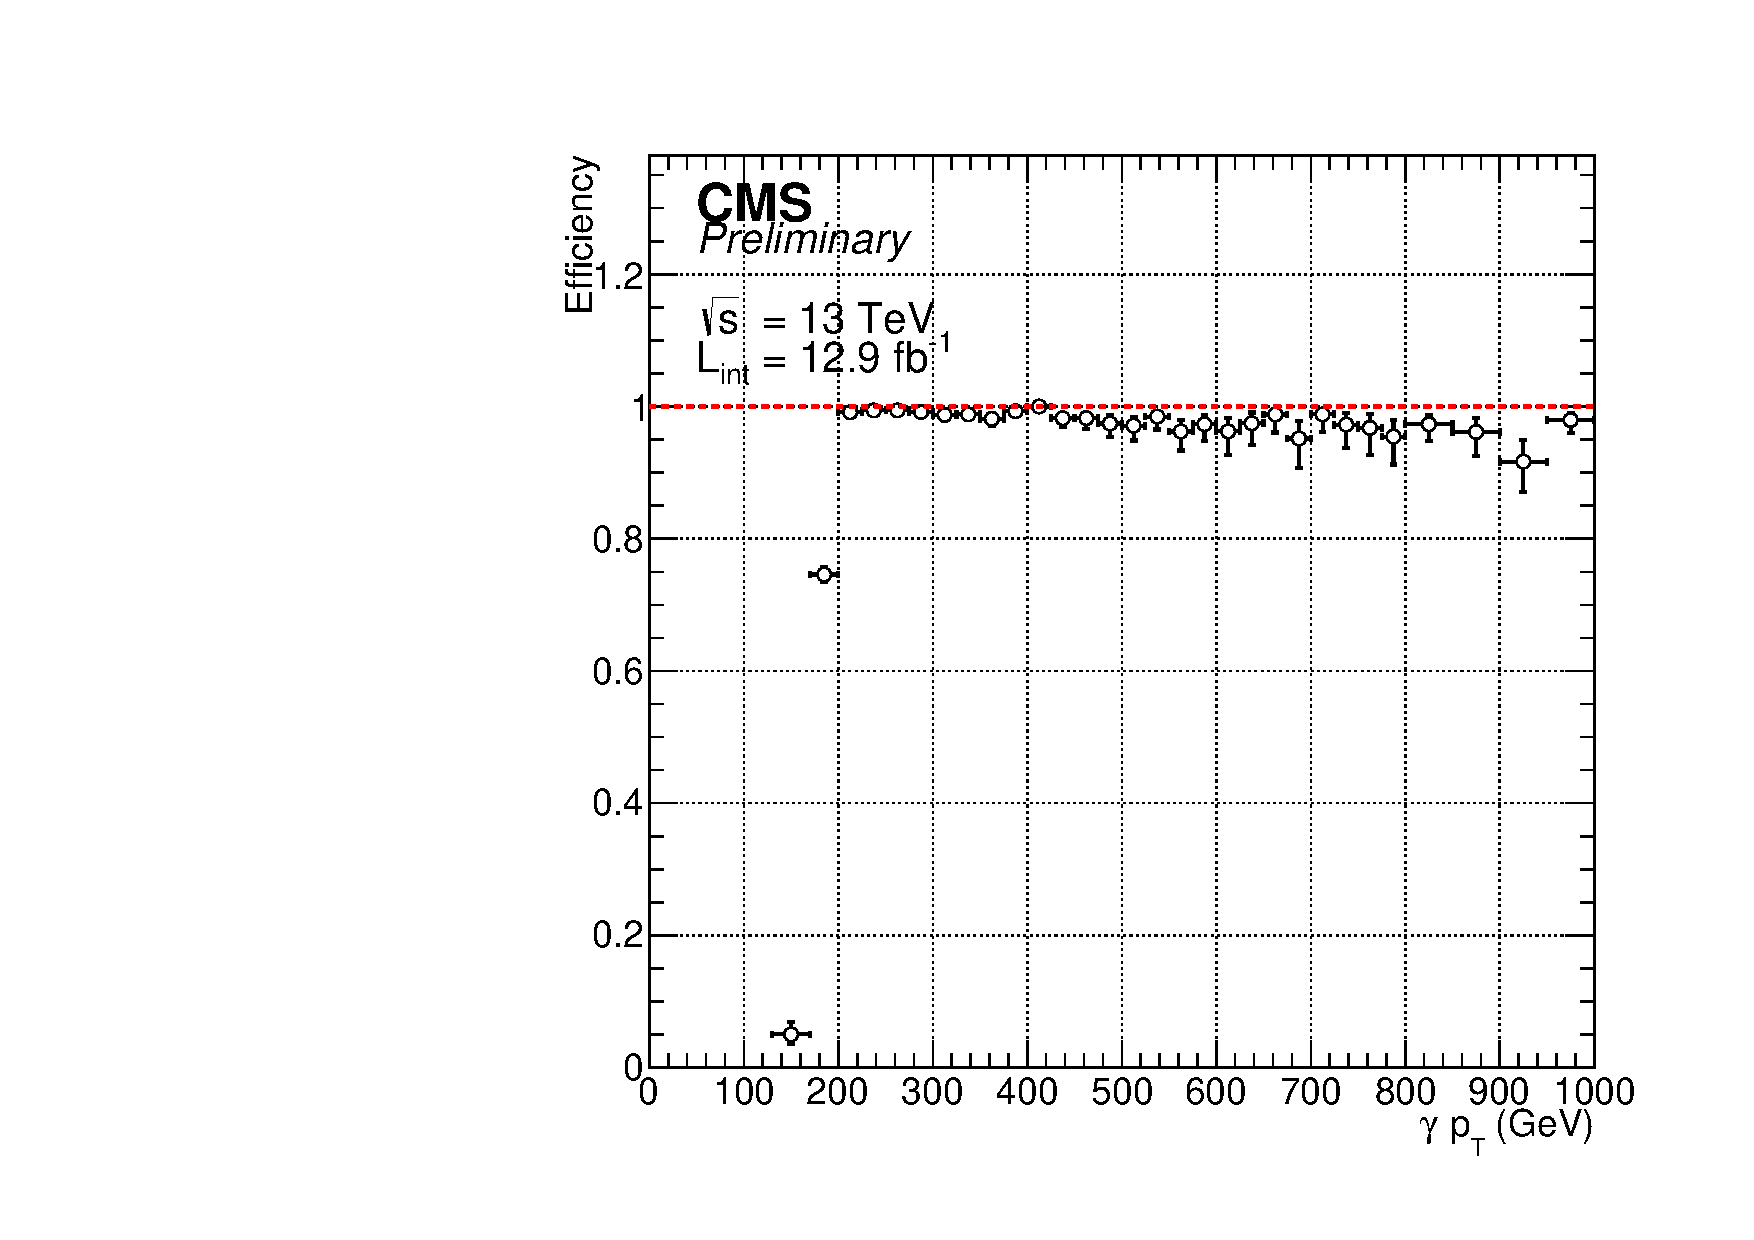
\includegraphics[width=0.4\textwidth]{figures/Trigger/Photon/HLT_Photon175_MoM_all_800to999999_gammapt}} ~~\
    \subfigure{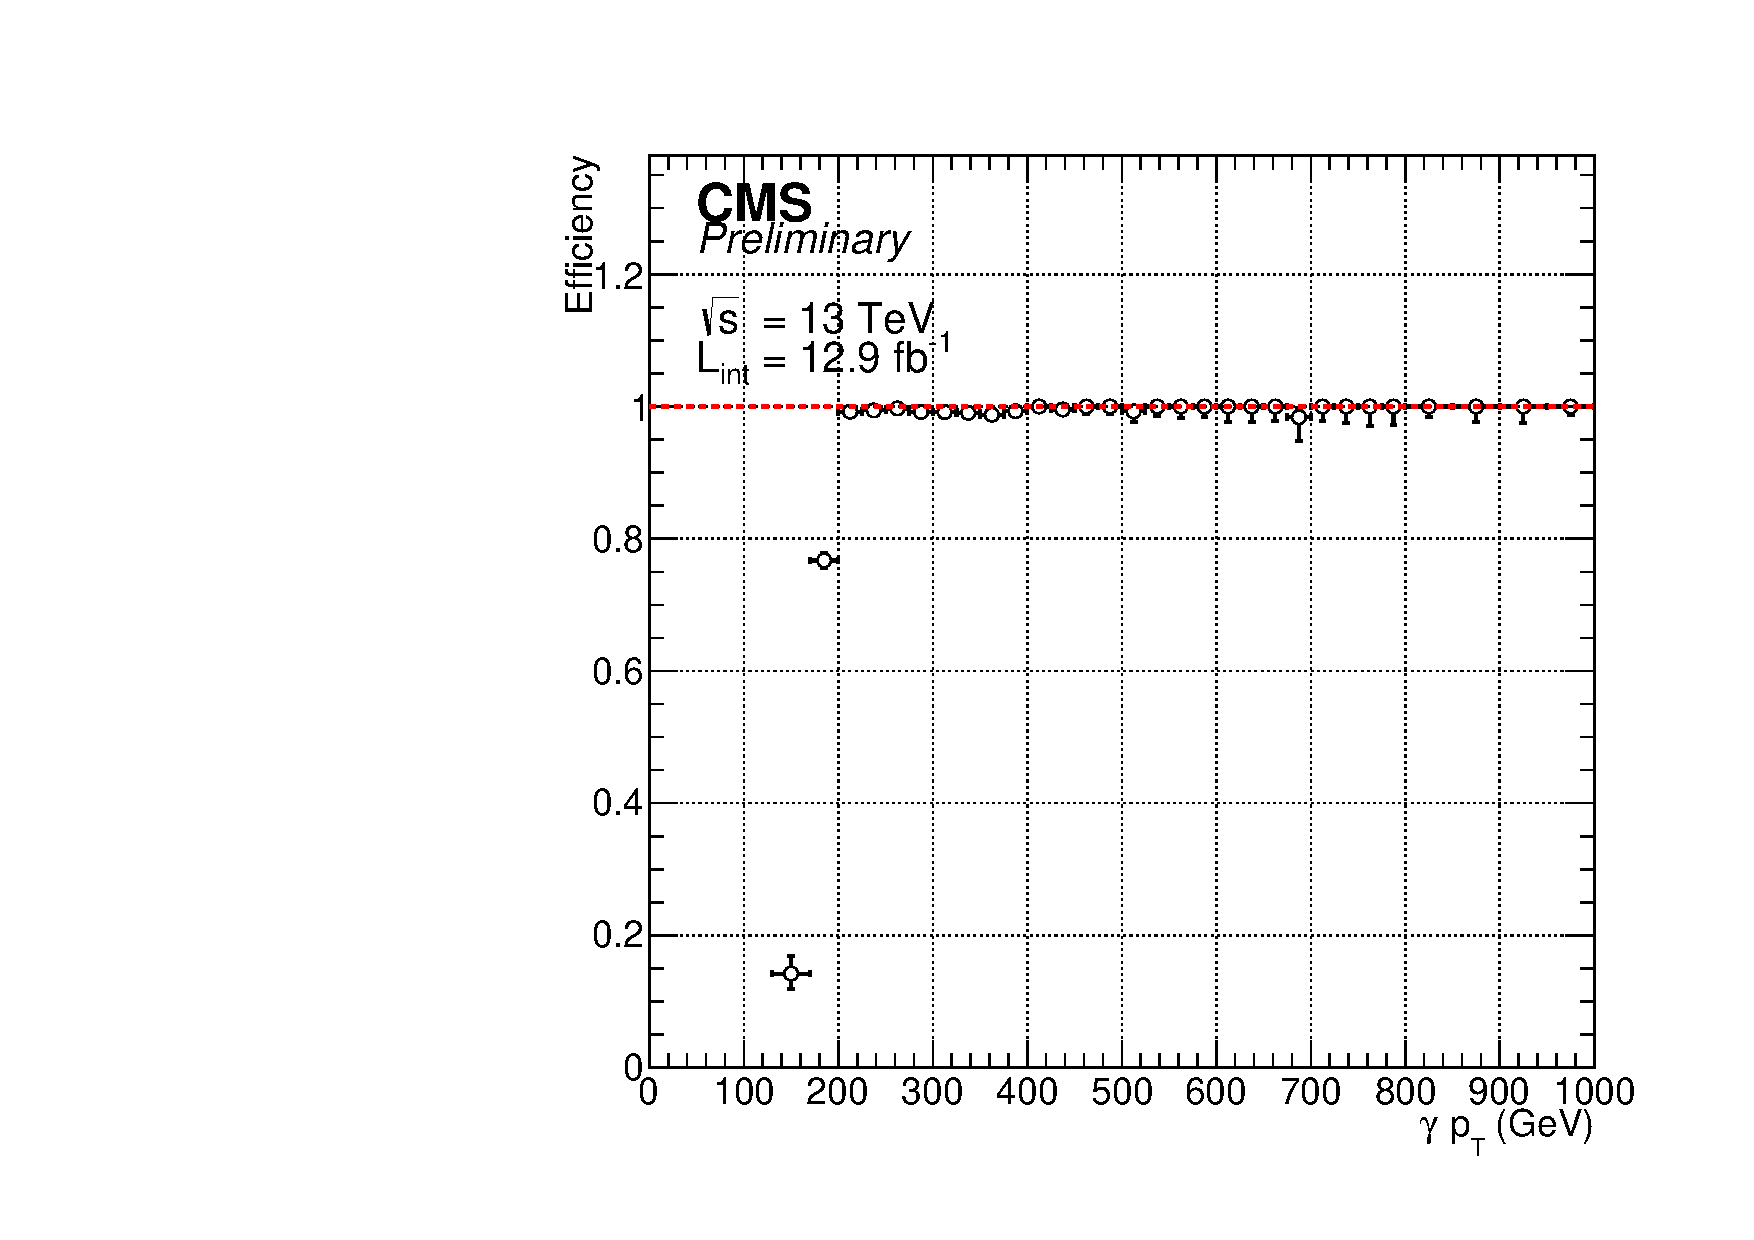
\includegraphics[width=0.4\textwidth]{figures/Trigger/Photon/HLT_PhotonECALHT800_MoM_all_800to999999_gammapt}} \\
    \caption{Trigger efficiency as a function of photon \Pt for Photon175 (left) and Photon175 OR ECALHT800 (right), measured with events in the JetHT data set passing the \gj control region selection. These are shown inclusive over \scalht (top) and for $\scalht > 800$~GeV (bottom).}
    \label{fig:photon_turnons}
  \end{center}
\end{figure}

\begin{figure}[h!]
  \begin{center}
    \subfigure{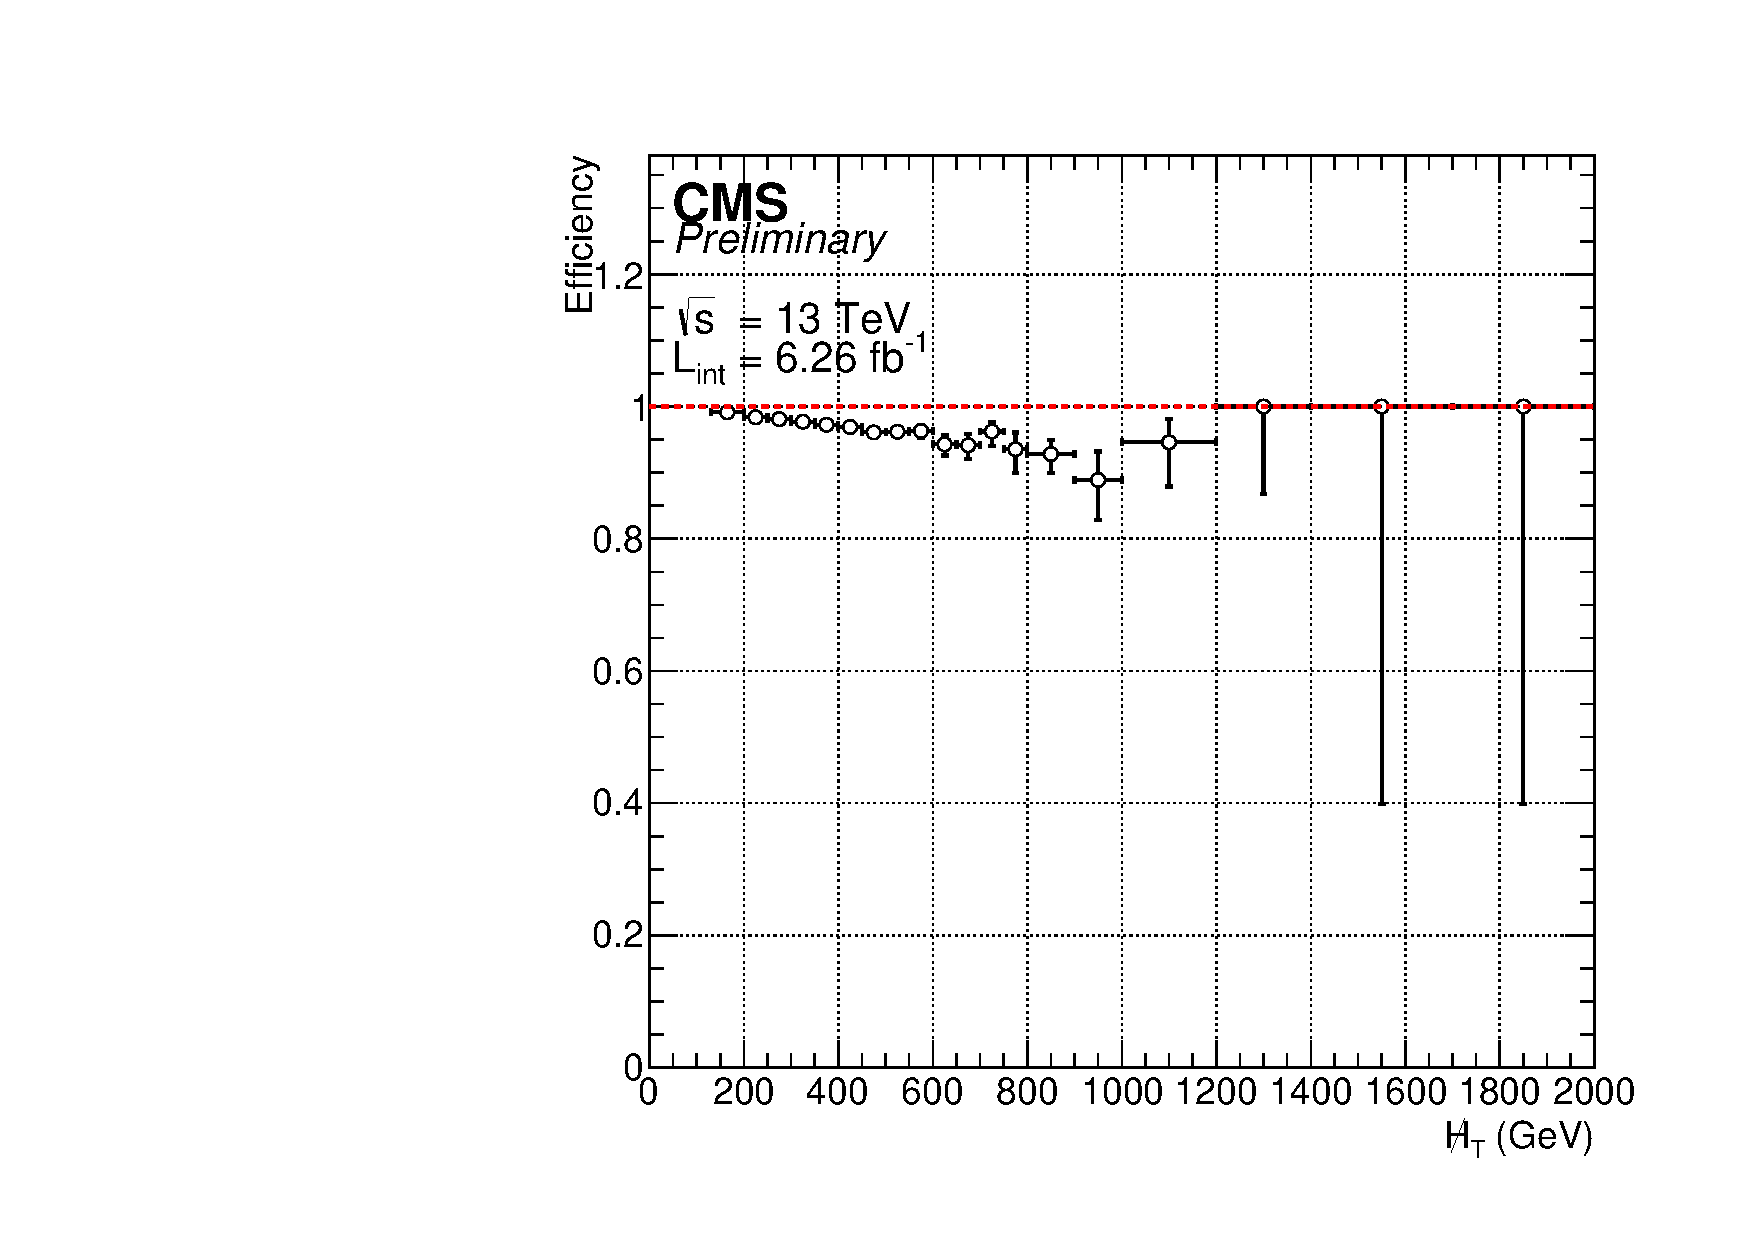
\includegraphics[width=0.4\textwidth]{figures/Trigger/Photon/HLT_Photon175_MoM_all_all_mht}} ~~\
    \subfigure{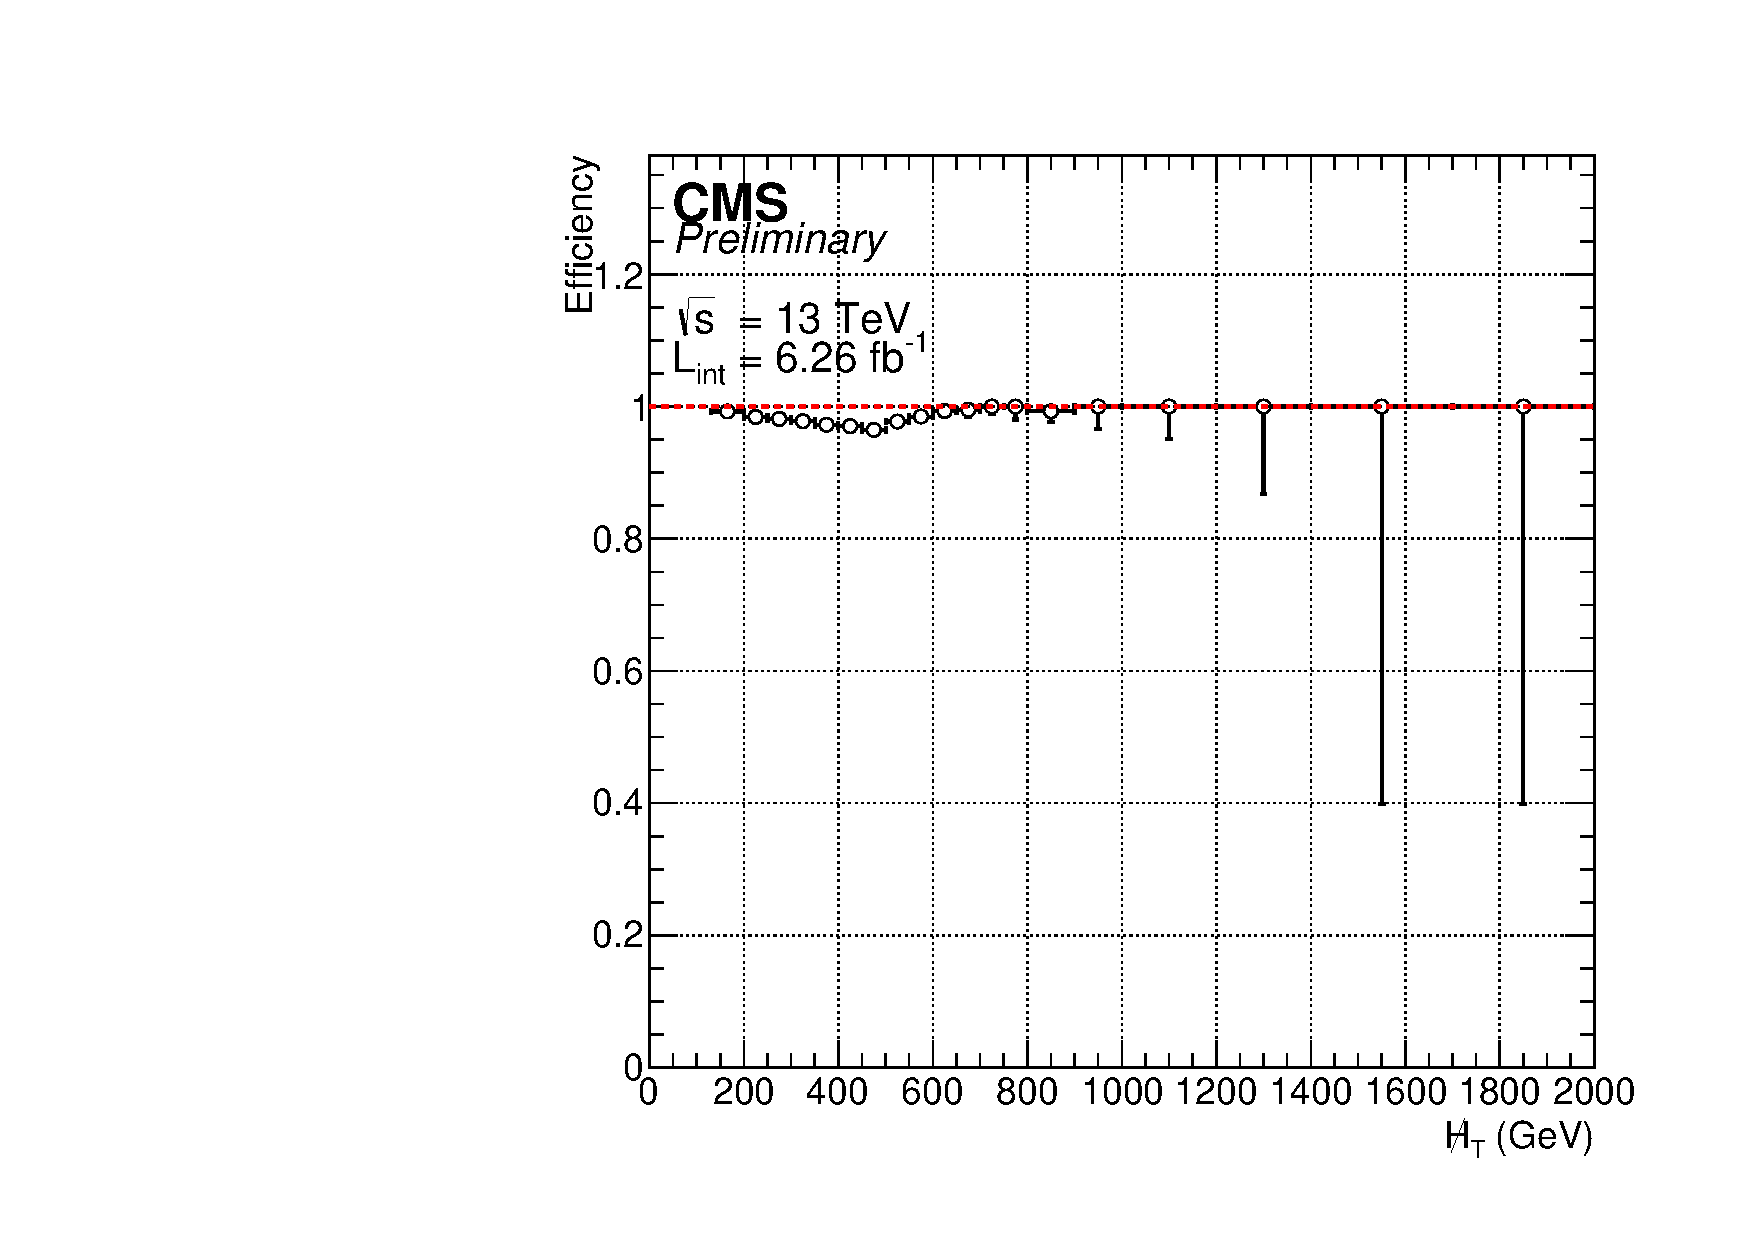
\includegraphics[width=0.4\textwidth]{figures/Trigger/Photon/HLT_PhotonECALHT800_MoM_all_all_mht}} \\
    \subfigure{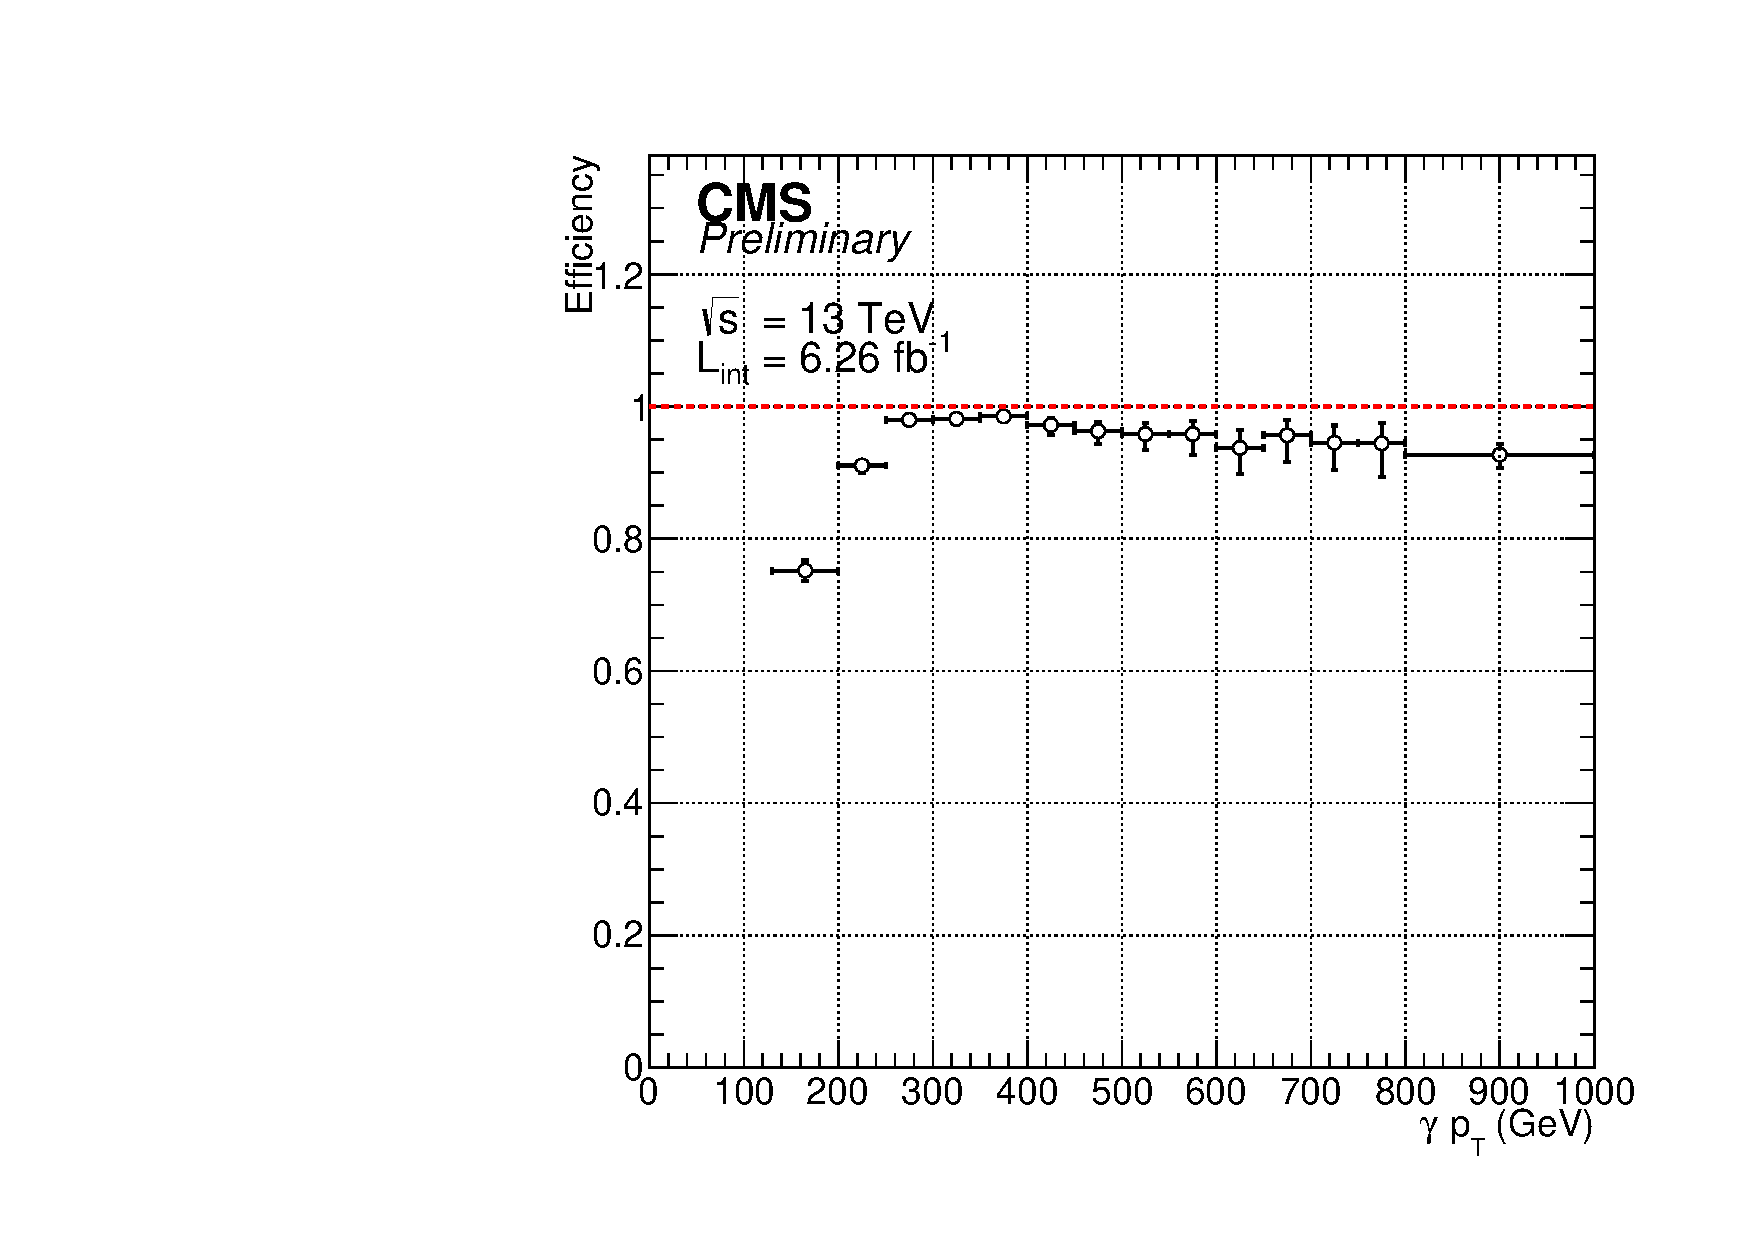
\includegraphics[width=0.4\textwidth]{figures/Trigger/Photon/HLT_Photon175_MoM_all_800to999999_mht}} ~~\
    \subfigure{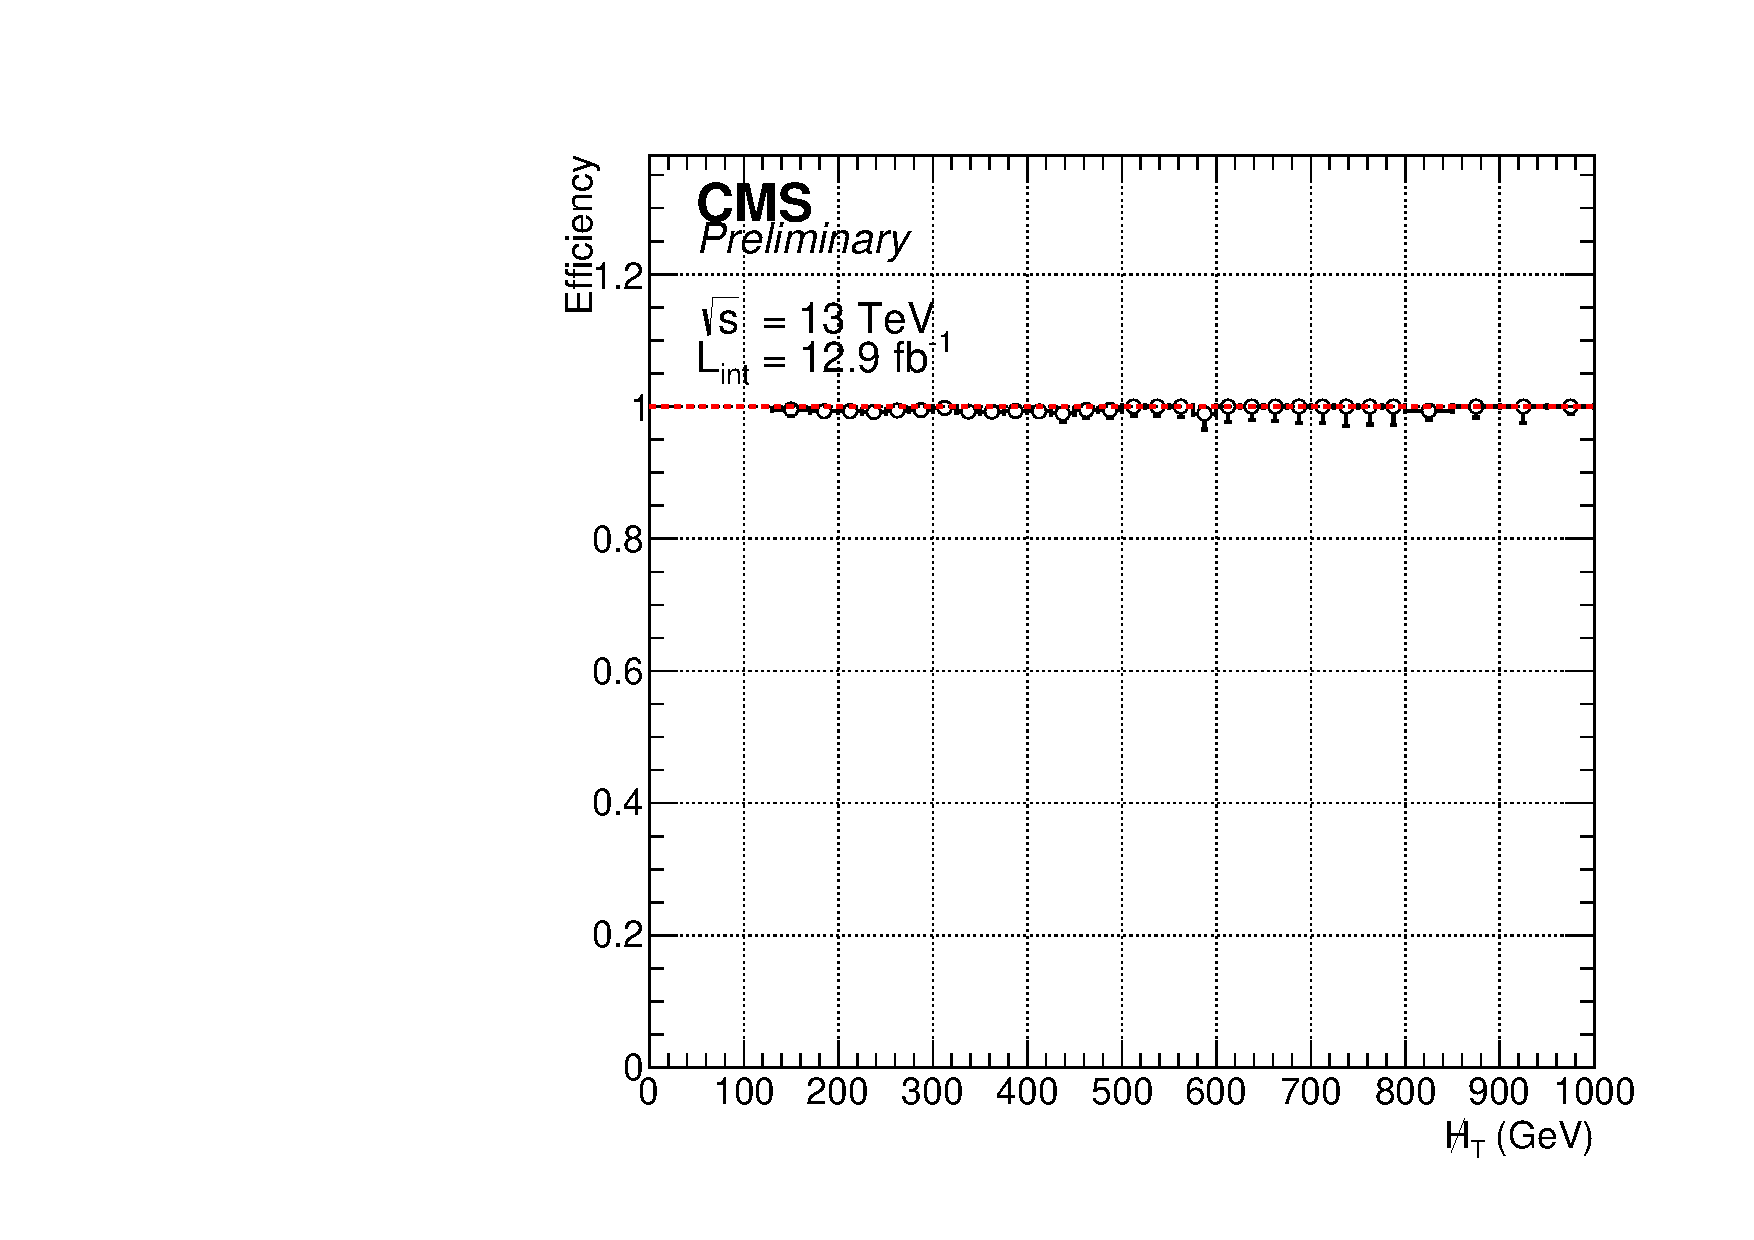
\includegraphics[width=0.4\textwidth]{figures/Trigger/Photon/HLT_PhotonECALHT800_MoM_all_800to999999_mht}} \\
    \caption{Trigger efficiency as a function of \mht for Photon175 (left) and Photon175 OR ECALHT800 (right), measured with events in the JetHT data set passing the \gj control region selection. These are shown inclusive over \scalht (top) and for $\scalht > 800$~GeV (bottom).}
    \label{fig:photon_turnons}
  \end{center}
\end{figure}


%The \ej and \eej control samples may be seeded by the \verb!HLT_Ele23_eta2p1_WPLoose_Gsf! trigger.

%The efficiency of the control triggers is measured with data-driven methods
%(provided by the relevant POG). The tag and probe method is used in the measurement of
%efficiencies of the muon and electron triggers and a loose photon reference trigger 
%is utilised in the measurement of the photon trigger efficiency. For the muon control 
%regions the emulated trigger bit in MC is used to simulate 
%the trigger, and efficiency corrections provided by the POG are applied. 
%An offline \Pt requirement of 200\GeV is made on the photon
%to ensure it is in the efficiency plateau of the trigger.



%%____________________________________________________________________________||
